% !BIB TS-program = biber

\RequirePackage[l2tabu,orthodox]{nag}
% TODO: decide if one-sided/two-sided
%\documentclass[headsepline,footsepline,footinclude=false,fontsize=11pt,paper=a4,listof=totoc,bibliography=totoc,BCOR=12mm,DIV=12]{scrbook} % two-sided
\documentclass[headsepline,footsepline,footinclude=false,oneside,fontsize=11pt,paper=a4,listof=totoc,bibliography=totoc]{scrbook} % one-sided
% TODO: change citation style in settings
\PassOptionsToPackage{table,svgnames,dvipsnames}{xcolor}

\usepackage[utf8]{inputenc}
\usepackage[T1]{fontenc}
\usepackage{lmodern}  
\usepackage[sc]{mathpazo}
\usepackage[provide=*, german, english]{babel}
\usepackage[autostyle]{csquotes}
\usepackage[%
  backend=biber,
  url=false,
  style=alphabetic,
  maxnames=4,
  minnames=3,
  maxbibnames=99,
  giveninits,
  uniquename=init]{biblatex} % TODO: adapt citation style
\usepackage{graphicx}
\usepackage{scrhack} % necessary for listings package
\usepackage{listings}
\usepackage{lstautogobble}
\usepackage{tikz}
\usepackage{pgfplots}
\usepackage{pgfplotstable}
\usepackage{booktabs}
\usepackage[final]{microtype}
\usepackage{caption}
\usepackage[printonlyused]{acronym}
\usepackage[hidelinks]{hyperref} % hidelinks removes colored boxes around references and links

\AtBeginDocument{%
	\hypersetup{
		pdftitle=\getTitle,
		pdfauthor=\getAuthor,
	}
}
\usepackage{ifthen}

% for fachschaft_print.pdf
\makeatletter
\if@twoside
	\typeout{TUM-Dev LaTeX-Thesis-Template: twoside}
\else
	\typeout{TUM-Dev LaTeX-Thesis-Template: oneside}
\fi
\makeatother

\addto\extrasamerican{
	\def\lstnumberautorefname{Line}
	\def\chapterautorefname{Chapter}
	\def\sectionautorefname{Section}
	\def\subsectionautorefname{Subsection}
	\def\subsubsectionautorefname{Subsubsection}
}

\addto\extrasngerman{
	\def\lstnumberautorefname{Zeile}
}

% Themes
\ifthenelse{\equal{\detokenize{dark}}{\jobname}}{%
  % Dark theme
  \newcommand{\bg}{black} % background
  \newcommand{\fg}{white} % foreground
  \usepackage[pagecolor=\bg]{pagecolor}
  \color{\fg}
}{%
  % Light theme
  \newcommand{\bg}{white} % background
  \newcommand{\fg}{black} % foreground
}

\bibliography{bibliography}
\addbibresource{bibliography.bib}


\setkomafont{disposition}{\normalfont\bfseries} % use serif font for headings
\linespread{1.05} % adjust line spread for mathpazo font

% Add table of contents to PDF bookmarks
\BeforeTOCHead[toc]{{\cleardoublepage\pdfbookmark[0]{\contentsname}{toc}}}

% Define TUM corporate design colors
% Taken from http://portal.mytum.de/corporatedesign/index_print/vorlagen/index_farben
\definecolor{TUMBlue}{HTML}{0065BD}
\definecolor{TUMSecondaryBlue}{HTML}{005293}
\definecolor{TUMSecondaryBlue2}{HTML}{003359}
\definecolor{TUMBlack}{HTML}{000000}
\definecolor{TUMWhite}{HTML}{FFFFFF}
\definecolor{TUMDarkGray}{HTML}{333333}
\definecolor{TUMGray}{HTML}{808080}
\definecolor{TUMLightGray}{HTML}{CCCCC6}
\definecolor{TUMAccentGray}{HTML}{DAD7CB}
\definecolor{TUMAccentOrange}{HTML}{E37222}
\definecolor{TUMAccentGreen}{HTML}{A2AD00}
\definecolor{TUMAccentLightBlue}{HTML}{98C6EA}
\definecolor{TUMAccentBlue}{HTML}{64A0C8}

% Settings for pgfplots
\pgfplotsset{compat=newest}
\pgfplotsset{
  % For available color names, see http://www.latextemplates.com/svgnames-colors
  cycle list={TUMBlue\\TUMAccentOrange\\TUMAccentGreen\\TUMSecondaryBlue2\\TUMDarkGray\\},
}

% Settings for lstlistings
\lstset{%
  basicstyle=\ttfamily,
  columns=fullflexible,
  autogobble,
  keywordstyle=\bfseries\color{TUMBlue},
  stringstyle=\color{TUMAccentGreen},
  captionpos=b
}


% TODO: change thesis information
\newcommand*{\getUniversity}{Technische Universität München}
\newcommand*{\getFaculty}{Informatics}
\newcommand*{\getDegree}{Informatics}
\newcommand*{\getSchool}{Computation, Information and Technology}
\newcommand*{\getTitle}{Portfolio Optimization with Gaussian Process Regression}
\newcommand*{\getTitleGer}{Titel der Abschlussarbeit}
\newcommand*{\getAuthor}{Xiyue ZHANG}
\newcommand*{\getDoctype}{Master's Thesis \ldots}
\newcommand*{\getSupervisor}{Prof. Dr. Hans-Jochim Bungartz}
\newcommand*{\getAdvisor}{Kislaya Ravi}
\newcommand*{\getSubmissionDate}{December 3rd}
\newcommand*{\getSubmissionLocation}{Munich}

\begin{document}

% Set page numbering to avoid "destination with the same identifier has been already used" warning for cover page.
% (see https://en.wikibooks.org/wiki/LaTeX/Hyperlinks#Problems_with_Links_and_Pages).
\pagenumbering{alpha}
\begin{titlepage}
  % HACK for two-sided documents: ignore binding correction for cover page.
  % Adapted from Markus Kohm's KOMA-Script titlepage=firstiscover handling.
  % See http://mirrors.ctan.org/macros/latex/contrib/koma-script/scrkernel-title.dtx,
  % \maketitle macro.
  \oddsidemargin=\evensidemargin\relax
  \textwidth=\dimexpr\paperwidth-2\evensidemargin-2in\relax
  \hsize=\textwidth\relax

  \centering

  \IfFileExists{logos/tum-\fg.pdf}{%
    \includegraphics[height=20mm]{logos/tum-\fg.pdf}
  }{%
    \vspace*{20mm}
  }

  \vspace{5mm}
  {\huge\MakeUppercase{School of \getSchool{} --- \getFaculty{}} \par}

  \vspace{5mm}
  {\large\MakeUppercase{\getUniversity{}} \par}

  \vspace{15mm}
  {\Large \getDoctype{} in \getDegree{} \par}

  \vspace{10mm}
  {\huge\bfseries \getTitle{} \par}

  \vspace{10mm}
  {\LARGE \getAuthor{}}

  \IfFileExists{logos/faculty-\fg.pdf}{%
    \vfill{}
    \includegraphics[height=20mm]{logos/faculty-\fg.pdf}
  }{}
\end{titlepage}


\frontmatter{}

\begin{titlepage}
  \centering

  \IfFileExists{logos/tum-\fg.pdf}{%
    \includegraphics[height=20mm]{logos/tum-\fg.pdf}
  }{%
    \vspace*{20mm}
  }

  \vspace{5mm}
  {\huge\MakeUppercase{School of \getSchool{} --- \getFaculty{}} \par}

  \vspace{5mm}
  {\large\MakeUppercase{\getUniversity{}} \par}

  \vspace{20mm}
  {\Large \getDoctype{} in \getDegree{} \par}

  \vspace{15mm}
  {\huge\bfseries \getTitle{} \par}

  \vspace{10mm}
  {\huge\bfseries \foreignlanguage{ngerman}{\getTitleGer{}} \par}

  \vspace{15mm}
  \begin{tabular}{l l}
    Author:          & \getAuthor{}         \\
    Supervisor:      & \getSupervisor{}     \\
    Advisor:         & \getAdvisor{}        \\
    Submission Date: & \getSubmissionDate{} \\
  \end{tabular}

  \IfFileExists{logos/faculty-\fg.pdf}{%
    \vfill{}
    \includegraphics[height=20mm]{logos/faculty-\fg.pdf}
  }{}
\end{titlepage}

\thispagestyle{empty}
\vspace*{0.8\textheight}
\noindent
I confirm that this \MakeLowercase{\getDoctype{}} is my own work and I have documented all sources and material used.

\vspace{15mm}
\noindent
\getSubmissionLocation{}, \getSubmissionDate{} \hspace{\fill} \getAuthor{}

\cleardoublepage{}

\addcontentsline{toc}{chapter}{Acknowledgments}
\thispagestyle{empty}

\vspace*{20mm}

\begin{center}
    {\usekomafont{sectioning}\usekomafont{section} Acknowledgments}
\end{center}

\vspace{10mm}

I would like to express my deepest gratitude to my advisor, Kislaya Ravi, for the invaluable guidance, support, and encouragement throughout the course of this thesis project. 
Ravi's expertise, insights, and unwavering commitment to excellence have been instrumental in shaping this work. 
His mentorship has not only guided me through the complexities of this research but has also inspired me to think critically and approach challenges with determination. 
This thesis would not have been possible without Ravi's patience, constructive feedback, and constant encouragement, which motivated me to strive for improvement at every step.
Additionally, I would like to extend my early congratulations and best wishes to Ravi for his upcoming marriage next February. I wish him and his partner a lifetime of happiness, love, and success.

I am also profoundly grateful to my parents for the time and effort they have always dedicated to supporting me, both physically and spiritually. Their unwavering love, encouragement, and belief in me have been a constant source of strength and inspiration. I am truly blessed to have such loving and supportive parents who have always encouraged me to pursue my dreams and never give up, even during the hardest times.

Lastly, I would like to extend my heartfelt thanks to Dr. Tian Weikun, who has provided invaluable assistance during the writing of this thesis. Thank you for believing in me and for your unwavering support throughout this journey.

\cleardoublepage{}

\chapter{\abstractname}

%TODO: Abstract

\microtypesetup{protrusion=false}
\tableofcontents{}
\microtypesetup{protrusion=true}

\mainmatter{}

% !TeX root = ../main.tex
% Add the above to each chapter to make compiling the PDF easier in some editors.

\chapter{Introduction}\label{chapter:introduction}

\section{Background and Motivation}
Citation test~\parencite{latex}.

Acronyms must be added in \texttt{main.tex} and are referenced using macros. The first occurrence is automatically replaced with the long version of the acronym, while all subsequent usages use the abbreviation.

E.g. \texttt{\textbackslash ac\{TUM\}, \textbackslash ac\{TUM\}} $\Rightarrow$ \ac{TUM}, \ac{TUM}

For more details, see the documentation of the \texttt{acronym} package\footnote{\url{https://ctan.org/pkg/acronym}}.


\subsection{Evolution of portfolio optimization techniques}
The field of portfolio optimization has undergone significant transformations since its inception in the mid-20th century, evolving from simple diversification principles to sophisticated mathematical models incorporating machine learning and artificial intelligence. 
This evolution reflects both the advancing computational capabilities and our deepening understanding of financial markets' complexity.


\paragraph{Classical Foundations (1950s-1960s)}
The modern era of portfolio optimization began with \parencite{markowitz1952portfolio}'s seminal paper ``Portfolio Selection,'' which laid the groundwork for Modern Portfolio Theory (MPT). Markowitz introduced several revolutionary concepts:

\begin{itemize}
    \item The mathematical formalization of diversification
    \item The mean-variance optimization framework
    \item The efficient frontier of optimal portfolios
    \item The fundamental relationship between risk and return
\end{itemize}

This work established the first rigorous mathematical framework for portfolio selection, earning Markowitz the Nobel Prize in Economics and fundamentally changing how practitioners approached portfolio management.

\paragraph{Early Developments (1960s-1980s)}
Building upon Markowitz's foundation, several crucial developments emerged:

\begin{enumerate}
    \item \textbf{Capital Asset Pricing Model (CAPM)}
    \begin{itemize}
        \item Developed by \parencite{sharpe1964capital}, \parencite{lintner1965security}, and \parencite{mossin1966equilibrium}
        \item Introduced systematic and unsystematic risk concepts
        \item Established the theoretical framework for asset pricing
        \item Created the foundation for risk-adjusted performance measures
    \end{itemize}

    \item \textbf{Single-Index Models}
    \begin{itemize}
        \item Simplified the estimation of covariance matrices
        \item Reduced computational complexity
        \item Introduced market beta as a risk measure
        \item Enhanced practical applicability of portfolio optimization
    \end{itemize}
\end{enumerate}

\paragraph{Advanced Optimization Era (1980s-2000s)}
The advent of increased computational power led to more sophisticated approaches:

\begin{enumerate}
    \item \textbf{Black-Litterman Model (1990s)}
    \begin{itemize}
        \item Incorporated investor views into the optimization process
        \item Addressed estimation error issues in mean-variance optimization
        \item Introduced Bayesian methods to portfolio optimization
        \item Provided more stable and intuitive portfolio allocations
    \end{itemize}

    \item \textbf{Risk-Based Portfolio Optimization}
    \begin{itemize}
        \item Development of risk parity strategies \parencite{qian2005risk}
        \item Introduction of alternative risk measures (VaR, CVaR)
        \item Focus on downside risk management
        \item Enhanced robustness to estimation errors
    \end{itemize}
\end{enumerate}

\paragraph{Modern Approaches (2000s-Present)}
Recent developments have focused on addressing classical methods' limitations:

\begin{enumerate}
    \item \textbf{Robust Optimization}
    \begin{itemize}
        \item Accounts for parameter uncertainty
        \item Provides protection against worst-case scenarios
        \item Incorporates estimation error in the optimization process
        \item Yields more stable portfolio allocations
    \end{itemize}

    \item \textbf{Dynamic Portfolio Optimization}
    \begin{itemize}
        \item Considers time-varying investment opportunities
        \item Incorporates transaction costs
        \item Accounts for changing market conditions
        \item Enables adaptive portfolio management
    \end{itemize}

    \item \textbf{Machine Learning Integration}
    \begin{itemize}
        \item Neural networks for return prediction \parencite{heaton2017deep}
        \item Support vector machines for risk assessment
        \item Reinforcement learning for portfolio management
        \item Gaussian processes for uncertainty quantification
    \end{itemize}
\end{enumerate}

\paragraph{Current Challenges and Future Directions}
Modern portfolio optimization faces several challenges:

\begin{enumerate}
    \item \textbf{Data Quality and Quantity}
    \begin{itemize}
        \item High-dimensional data processing
        \item Non-stationary market conditions
        \item Alternative data integration
        \item Real-time data processing requirements
    \end{itemize}

    \item \textbf{Model Complexity}
    \begin{itemize}
        \item Balance between model sophistication and robustness
        \item Computational efficiency
        \item Interpretability of results
        \item Parameter stability
    \end{itemize}

    \item \textbf{Implementation Challenges}
    \begin{itemize}
        \item Transaction costs
        \item Market impact
        \item Regulatory constraints
        \item Operational considerations
    \end{itemize}
\end{enumerate}

The field continues to evolve with emerging technologies and methodologies:

\begin{enumerate}
    \item \textbf{Artificial Intelligence Applications}
    \begin{itemize}
        \item Deep learning for market prediction
        \item Natural language processing for sentiment analysis
        \item Alternative data processing
        \item Automated portfolio rebalancing
    \end{itemize}

    \item \textbf{Advanced Risk Management}
    \begin{itemize}
        \item Tail risk hedging
        \item Dynamic risk allocation
        \item Scenario analysis
        \item Real-time risk monitoring
    \end{itemize}

    \item \textbf{Sustainability Integration}
    \begin{itemize}
        \item ESG factors in optimization
        \item Climate risk consideration
        \item Impact investing metrics
        \item Sustainable portfolio construction
    \end{itemize}
\end{enumerate}

This evolution of portfolio optimization techniques sets the stage for our research, which builds upon these foundations while incorporating modern machine learning approaches, specifically Gaussian Process Regression, to address current challenges in portfolio optimization.


\subsection{Role of machine learning in financial forecasting}
Machine learning (ML) has gained significant traction in financial markets due to its ability to analyze vast amounts of data and identify complex patterns that traditional models may overlook.
In particular, Gaussian Process Regression (GPR) has emerged as a powerful tool for time-series forecasting, offering a flexible framework for capturing non-linear relationships and uncertainty in predictions.

\subsection{Challenges in time-series forecasting and traditional portfolio optimization methods}
Despite the advancements in ML techniques, predicting asset returns remains a challenging task due to the inherent volatility and non-stationarity of financial markets.
Moreover, traditional portfolio optimization methods, while theoretically elegant, often face significant practical challenges in implementation. These challenges primarily stem from the difficulty in accurately estimating input parameters and the inherent uncertainty in financial time-series forecasting. 
This section examines these challenges and introduces how Gaussian Process Regression (GPR) provides a novel approach to addressing them.

\paragraph{Parameter Estimation Challenges in Modern Portfolio Theory}
Modern Portfolio Theory (MPT), despite its theoretical elegance, relies heavily on accurate estimation of key parameters:
The practical implementation of MPT is fundamentally constrained by the difficulty in estimating volatility, arguably the most critical parameter in portfolio optimization. Traditional approaches to volatility estimation rely heavily on historical data, assuming that past patterns will persist into the future. However, financial markets are dynamic systems characterized by regime changes, varying volatility clusters, and complex interdependencies that make such assumptions problematic. Historical volatility estimates are inherently backward-looking and highly sensitive to the chosen estimation window, leading to potentially misleading inputs for portfolio optimization.

Moreover, the challenge extends beyond simple volatility estimation. The correlation structure between assets, another crucial input for MPT, exhibits time-varying properties that are difficult to capture using conventional methods. During periods of market stress, these correlations often shift dramatically, invalidating historical estimates precisely when accurate risk assessment is most critical. The dimensionality of this problem grows quadratically with the number of assets, making it particularly challenging for large, diversified portfolios.

\begin{itemize}
    \item \textbf{Volatility Estimation}
    \begin{itemize}
        \item Historical volatility may not reflect future risk
        \item Sample estimates are sensitive to the chosen time window
        \item Regime changes can invalidate historical estimates
        \item Heteroskedasticity in financial time series complicates estimation
    \end{itemize}

    \item \textbf{Expected Returns}
    \begin{itemize}
        \item Notoriously difficult to estimate accurately
        \item High sensitivity to estimation errors
        \item Time-varying nature of expected returns
        \item Impact of market regimes on return distributions
    \end{itemize}

    \item \textbf{Correlation Structure}
    \begin{itemize}
        \item Dynamic nature of asset correlations
        \item Curse of dimensionality in large portfolios
        \item Instability during market stress periods
        \item Computational challenges in high dimensions
    \end{itemize}
\end{itemize}

\paragraph{Limitations of Traditional Forecasting Methods}
Traditional forecasting approaches in finance have predominantly relied on methods that provide point estimates, failing to capture the inherent uncertainty in financial predictions. These methods often make strong assumptions about the underlying data distribution and struggle to adapt to the non-linear, non-stationary nature of financial time series. ARIMA models, exponential smoothing, and other classical approaches, while mathematically tractable, often fall short in capturing the complex dynamics of financial markets.

A fundamental limitation of these traditional approaches is their rigidity in handling uncertainty. Point forecasts, even when accompanied by confidence intervals based on historical volatility, fail to capture the dynamic nature of prediction uncertainty. This limitation becomes particularly problematic in portfolio optimization, where understanding the reliability of forecasts is as important as the forecasts themselves.

Conventional approaches to financial time-series forecasting exhibit several limitations:

\begin{enumerate}
    \item \textbf{Point Estimates}
    \begin{itemize}
        \item Traditional methods often provide single-point forecasts
        \item Lack of uncertainty quantification
        \item Limited ability to capture prediction confidence
        \item Insufficient information for risk management
    \end{itemize}

    \item \textbf{Model Rigidity}
    \begin{itemize}
        \item Assumption of specific probability distributions
        \item Difficulty in capturing non-linear relationships
        \item Limited adaptation to changing market conditions
        \item Oversimplification of complex market dynamics
    \end{itemize}

    \item \textbf{Data Requirements}
    \begin{itemize}
        \item Need for large historical datasets
        \item Sensitivity to outliers and noise
        \item Challenge of incorporating multiple data sources
        \item Difficulty in handling missing data
    \end{itemize}
\end{enumerate}

\paragraph{Advantages of Gaussian Process Regression}
Our research proposes GPR as a solution to these challenges, offering several key advantages:

\begin{enumerate}
    \item \textbf{Probabilistic Framework}
    \begin{itemize}
        \item Natural uncertainty quantification
        \item Automatic volatility estimation through posterior variance
        \item Capture of prediction confidence intervals
        \item Robust handling of noise in financial data
    \end{itemize}

    \item \textbf{Flexible Modeling}
    \begin{itemize}
        \item Non-parametric approach avoiding distributional assumptions
        \item Ability to capture complex non-linear relationships
        \item Automatic complexity adjustment through kernel selection
        \item Incorporation of prior knowledge through kernel design
    \end{itemize}

    \item \textbf{Parameter Estimation}
    \begin{itemize}
        \item Direct modeling of volatility through posterior variance
        \item Joint estimation of returns and risk
        \item Principled handling of uncertainty
        \item Adaptive to changing market conditions
    \end{itemize}
\end{enumerate}

\paragraph{Addressing Traditional Limitations}
Our GPR-based approach specifically addresses the key limitations of MPT:

\begin{equation}
    \sigma_{GPR}^2(x_*) = k(x_*, x_*) - k(x_*, X)[K(X,X) + \sigma_n^2I]^{-1}k(X, x_*)
    \label{eq:gpr_variance}
\end{equation}

Where $\sigma_{GPR}^2(x_*)$ represents the posterior variance at prediction point $x_*$, providing a direct estimate of volatility that:

\begin{itemize}
    \item Naturally accounts for uncertainty in predictions
    \item Adapts to local data density and quality
    \item Provides time-varying volatility estimates
    \item Incorporates both local and global market information
\end{itemize}

The GPR approach offers several fundamental advantages over traditional methods. Unlike historical volatility estimates that require arbitrary window selection, GPR's volatility estimates emerge naturally from the probabilistic learning process. The method adapts automatically to different market regimes through its kernel function, which can capture both long-term trends and short-term fluctuations in market behavior.

Furthermore, GPR's non-parametric nature frees it from restrictive assumptions about return distributions. The method can capture complex, non-linear patterns in the data while maintaining the ability to quantify uncertainty in its predictions. This combination of flexibility and uncertainty awareness makes it particularly well-suited for financial applications where both accuracy and risk assessment are crucial.


\paragraph{Implications for Portfolio Optimization}
The GPR framework transforms the traditional portfolio optimization problem by:
The integration of GPR into portfolio optimization transforms the traditional MPT framework by providing more reliable and dynamic parameter estimates. By directly modeling the uncertainty in our predictions, we can make more informed portfolio allocation decisions that account for both expected returns and our confidence in those expectations. This approach naturally leads to more robust portfolios that adapt to changing market conditions while maintaining a principled approach to risk management.

The significance of this advancement cannot be overstated. By addressing one of the fundamental criticisms of MPT – the difficulty of accurately estimating volatility – our GPR-based approach bridges the gap between theoretical elegance and practical applicability. This enhancement makes MPT more reliable and useful for real-world portfolio management, where accurate risk assessment is crucial for maintaining stable, long-term investment performance.


\section{Research Objectives}
The primary objective of this study is to develop a predictive portfolio optimization framework that leverages Gaussian Process Regression (GPR) for time-series forecasting in financial markets. 
By integrating advanced predictive modeling with strategic asset allocation, the study aims to enhance investment performance through informed decision-making. 
The specific objectives are as follows:

\begin{enumerate}
    \item \textbf{Develop and Validate GPR Models for Asset Return Prediction}
    \begin{itemize}
        \item \emph{Model Construction:} Build individual GPR models to forecast future returns of selected assets, including forex, gold, Bitcoin, and various stocks.
        \item \emph{Feature Engineering:} Utilize historical one-month returns and time as input features to capture both market dynamics and temporal patterns.
        \item \emph{Model Updating:} Implement an iterative training process where models are updated daily with new market data to ensure predictions remain current and adaptive.
    \end{itemize}
    
    \item \textbf{Integrate GPR Predictions into Portfolio Optimization Strategies}
    \begin{itemize}
        \item \emph{Expected Returns and Volatilities:} Extract predicted returns and associated volatilities from the GPR models for use in portfolio construction.
        \item \emph{Strategy Formulation:} Design multiple optimization strategies---Maximum Return, Minimum Volatility, Maximum Sharpe Ratio, and a Dynamic Strategy---based on the GPR outputs.
    \end{itemize}
    
    \item \textbf{Develop a Dynamic Portfolio Optimization Strategy}
    \begin{itemize}
        \item \emph{Probabilistic Assessment:} Calculate the probability distribution of next-day cumulative portfolio returns using the predicted normal distribution of asset returns.
        \item \emph{Threshold-Based Decision Making:} Establish a threshold probability to decide when to reallocate the portfolio for maximizing returns versus holding the current positions.
        \item \emph{Adaptive Allocation:} Enable the portfolio to adapt dynamically to changing market conditions by selectively applying the Maximum Return Strategy based on probabilistic forecasts.
    \end{itemize}
    
    \item \textbf{Evaluate and Compare the Performance of Optimization Strategies}
    \begin{itemize}
        \item \emph{Backtesting Framework:} Conduct backtesting over a historical period using real market data to assess the strategies' performance.
        \item \emph{Incorporation of Transaction Costs:} Include realistic transaction fees in the evaluation to account for the costs associated with portfolio rebalancing.
        \item \emph{Performance Metrics:} Measure total returns, portfolio volatility, Sharpe ratios, and transaction costs to provide a comprehensive performance analysis.
    \end{itemize}
    
    \item \textbf{Demonstrate the Effectiveness of the Dynamic Strategy}
    \begin{itemize}
        \item \emph{Performance Analysis:} Analyze the results to determine if the Dynamic Strategy achieves higher returns and lower transaction costs compared to traditional strategies.
        \item \emph{Risk Management:} Assess how the Dynamic Strategy balances the trade-off between pursuing higher returns and minimizing risks and costs.
        \item \emph{Statistical Significance:} Use statistical methods to verify the significance of the observed performance differences among the strategies.
    \end{itemize}
    
    \item \textbf{Contribute to the Field of Predictive Portfolio Optimization}
    \begin{itemize}
        \item \emph{Innovative Approach:} Present a novel integration of GPR-based forecasting with adaptive portfolio optimization strategies.
        \item \emph{Practical Implications:} Provide insights and recommendations for practitioners on implementing dynamic, data-driven approaches in portfolio management.
        \item \emph{Foundation for Future Research:} Establish a basis for further exploration into advanced predictive models and adaptive strategies in financial optimization.
    \end{itemize}
\end{enumerate}

By achieving these objectives, the study seeks to demonstrate that incorporating sophisticated predictive models like GPR into portfolio optimization can significantly enhance investment outcomes. The findings aim to contribute valuable knowledge to the field of quantitative finance, particularly in the areas of time-series forecasting and dynamic asset allocation.

\subsection{Research Contributions}

This study makes several significant contributions to the field of predictive portfolio optimization and quantitative finance. The key research contributions are outlined below:

\begin{enumerate}
    \item \textbf{Novel Integration of Gaussian Process Regression with Dynamic Portfolio Optimization}

    This research presents a unique integration of Gaussian Process Regression (GPR) models with dynamic portfolio optimization strategies. By employing GPR for time-series forecasting, we capture complex, non-linear relationships in financial data, enhancing the accuracy of return predictions. The integration facilitates a more responsive and informed portfolio allocation process, adapting to market changes in real-time.

    \item \textbf{Probabilistic Approach to Strategy Selection}

    We introduce a probabilistic framework for strategy selection within the portfolio optimization process. By calculating the probability distribution of future cumulative returns, the Dynamic Strategy makes informed decisions on whether to reallocate the portfolio based on a predefined threshold. This approach incorporates uncertainty and risk directly into the decision-making process, allowing for a more nuanced and adaptive investment strategy.

    \item \textbf{Practical Implementation Considering Transaction Costs}

    The study emphasizes practical applicability by incorporating realistic transaction costs into the optimization and backtesting processes. By accounting for these costs, we provide a more accurate assessment of the strategies' net performance. This consideration is crucial for real-world portfolio management, where transaction fees can significantly impact returns, especially in high-frequency trading environments.

    \item \textbf{Comparative Analysis of Different Optimization Strategies}

    We conduct a comprehensive comparative analysis of multiple portfolio optimization strategies, including Maximum Return, Minimum Volatility, Maximum Sharpe Ratio, and the proposed Dynamic Strategy. By evaluating these strategies under the same conditions and performance metrics, we provide valuable insights into their relative effectiveness. This analysis helps identify the strengths and limitations of each approach, guiding practitioners in selecting appropriate strategies based on their investment goals and risk tolerance.

\end{enumerate}

These contributions collectively advance the understanding of how advanced predictive models and adaptive strategies can be effectively combined to enhance portfolio performance. The novel methodologies and findings offer practical benefits for portfolio managers and lay the groundwork for future research in predictive asset allocation.




\begin{table}[htpb]
  \caption[Example table]{An example for a simple table.}
  \centering
  \begin{tabular}{l l l l}
    \toprule
      A & B & C & D \\
    \midrule
      1 & 2 & 1 & 2 \\
      2 & 3 & 2 & 3 \\
    \bottomrule
  \end{tabular}
\end{table}

\begin{figure}[htpb]
  \centering
  % This should probably go into a file in figures/
  \begin{tikzpicture}[node distance=3cm]
    \node (R0) {$R_1$};
    \node (R1) [right of=R0] {$R_2$};
    \node (R2) [below of=R1] {$R_4$};
    \node (R3) [below of=R0] {$R_3$};
    \node (R4) [right of=R1] {$R_5$};

    \path[every node]
      (R0) edge (R1)
      (R0) edge (R3)
      (R3) edge (R2)
      (R2) edge (R1)
      (R1) edge (R4);
  \end{tikzpicture}
  \caption[Example drawing]{An example for a simple drawing.}
\end{figure}

\begin{figure}[htpb]
  \centering

  \pgfplotstableset{col sep=&, row sep=\\}
  % This should probably go into a file in data/
  \pgfplotstableread{
    a & b    \\
    1 & 1000 \\
    2 & 1500 \\
    3 & 1600 \\
  }\exampleA
  \pgfplotstableread{
    a & b    \\
    1 & 1200 \\
    2 & 800 \\
    3 & 1400 \\
  }\exampleB
  % This should probably go into a file in figures/
  \begin{tikzpicture}
    \begin{axis}[
        ymin=0,
        legend style={legend pos=south east},
        grid,
        thick,
        ylabel=Y,
        xlabel=X
      ]
      \addplot table[x=a, y=b]{\exampleA};
      \addlegendentry{Example A};
      \addplot table[x=a, y=b]{\exampleB};
      \addlegendentry{Example B};
    \end{axis}
  \end{tikzpicture}
  \caption[Example plot]{An example for a simple plot.}
\end{figure}

\begin{figure}[htpb]
  \centering
  \begin{tabular}{c}
  \begin{lstlisting}[language=SQL]
    SELECT * FROM tbl WHERE tbl.str = "str"
  \end{lstlisting}
  \end{tabular}
  \caption[Example listing]{An example for a source code listing.}
\end{figure}

!TeX root = ../main.tex
% Add the above to each chapter to make compiling the PDF easier in some editors.

\chapter{Previous Literature}\label{chapter:previous literature}

\section{Theoretical Framework}

This chapter discusses the fundamental theories underpinning the study, focusing on portfolio optimization and \ac{GPR}. Understanding these theories is essential for developing the predictive portfolio optimization framework proposed in this research.

\subsection{Portfolio Optimization Theory}

Portfolio optimization is a cornerstone of modern finance, aiming to allocate assets in a way that balances expected returns against risk. The foundational theory in this domain is the \ac{MPT}, introduced by Harry Markowitz in 1952 \cite{markowitz1952portfolio}.

\subsubsection{Modern Portfolio Theory (MPT)}

\ac{MPT} posits that investors can construct an optimal portfolio that offers the maximum expected return for a given level of risk or, equivalently, the minimum risk for a given level of expected return. The key assumptions of MPT are:

\begin{itemize}
    \item Investors are rational and risk-averse, preferring higher returns and lower risk.
    \item Markets are efficient, and all investors have access to the same information.
    \item Asset returns are normally distributed and can be described by their mean (expected return) and variance (risk).
\end{itemize}

\paragraph{Expected Return and Risk}

The expected return of a portfolio, $E[R_p]$, is the weighted sum of the expected returns of the individual assets:

\begin{equation}
    E[R_p] = \sum_{i=1}^{n} w_i E[R_i],
\end{equation}

where $w_i$ is the weight of asset $i$ in the portfolio, $E[R_i]$ is the expected return of asset $i$, and $n$ is the total number of assets.

The portfolio variance, $\sigma_p^2$, representing risk, is given by:

\begin{equation}
    \sigma_p^2 = \sum_{i=1}^{n} \sum_{j=1}^{n} w_i w_j \sigma_{ij},
\end{equation}

where $\sigma_{ij}$ is the covariance between asset $i$ and asset $j$. The standard deviation $\sigma_p$ is the square root of the variance.

\paragraph{Efficient Frontier}

The set of optimal portfolios that offer the highest expected return for a given level of risk forms the \textit{Efficient Frontier}. Portfolios on the efficient frontier are considered optimal, as no other portfolios offer higher returns for the same risk level.

\begin{figure}[h]
    \centering
    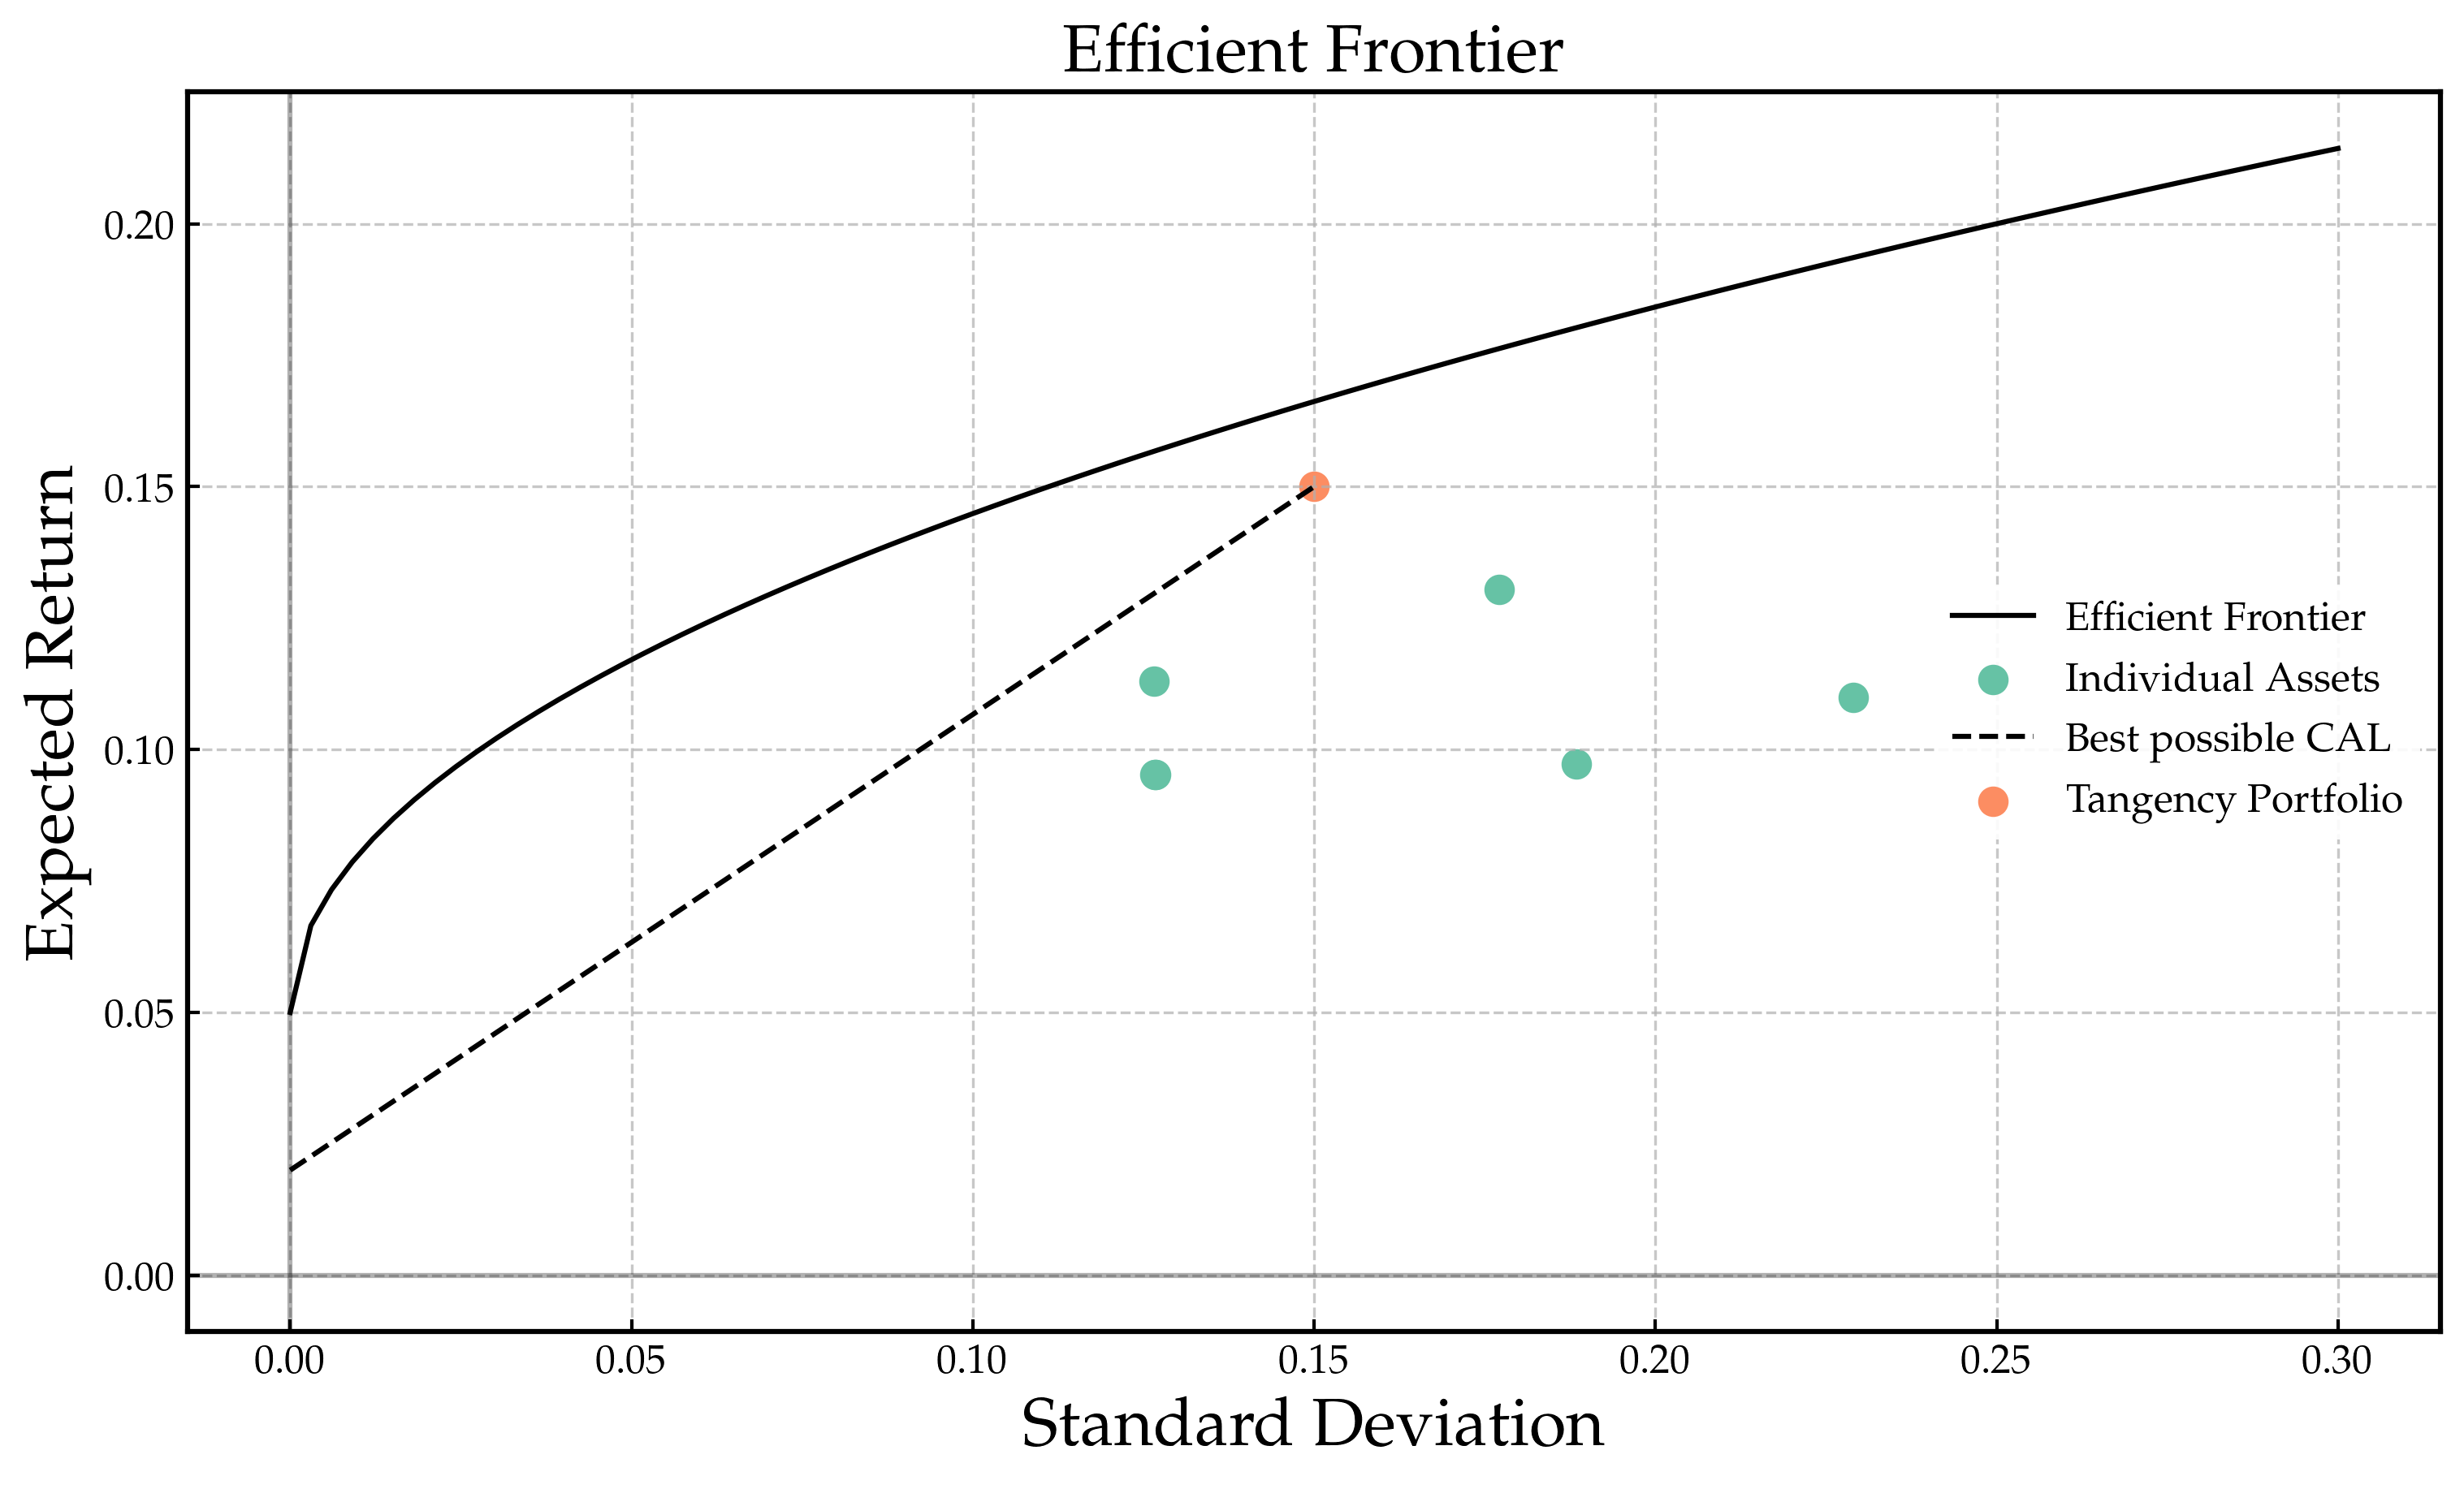
\includegraphics[width=0.6\textwidth]{figures/efficient_frontier.png}
    \caption{Efficient Frontier in Mean-Variance Space}
    \label{fig:efficient_frontier}
\end{figure}

\paragraph{Mean-Variance Optimization}

Mean-variance optimization involves solving for the portfolio weights that minimize the portfolio variance for a given expected return. The optimization problem can be formulated as:

\begin{equation}
\begin{aligned}
    \min_{\mathbf{w}} \quad & \mathbf{w}^T \boldsymbol{\Sigma} \mathbf{w} \\[1ex]
    \text{subject to} \quad & \mathbf{w}^T \mathbf{E} = E_p, \\[1ex]
    & \sum_{i=1}^{n} w_i = 1, \\[1ex]
    & w_i \geq 0, \quad i = 1,\ldots,n,
\end{aligned}
\end{equation}

where:
\begin{itemize}
    \item $\mathbf{w} \in \mathbb{R}^n$ is the vector of asset weights
    \item $\boldsymbol{\Sigma} \in \mathbb{R}^{n \times n}$ is the covariance matrix of asset returns
    \item $\mathbf{E} \in \mathbb{R}^n$ is the vector of expected asset returns
    \item $E_p \in \mathbb{R}$ is the desired expected portfolio return
\end{itemize}
\subsubsection{Risk-Return Trade-off and the Sharpe Ratio}

Investors seek to maximize returns while minimizing risk. The \textit{Sharpe Ratio}, introduced by William F. Sharpe \cite{sharpe1966mutual}, measures the risk-adjusted return of a portfolio:

\begin{equation}
    S = \frac{E[R_p] - R_f}{\sigma_p},
\end{equation}

where $R_f$ is the risk-free rate. A higher Sharpe Ratio indicates a more favorable risk-return trade-off.

\subsubsection{Portfolio Optimization Strategies}

Various strategies exist for portfolio optimization, each with different objectives and constraints:

\begin{itemize}
    \item \textbf{Maximum Return Strategy}: Focuses on maximizing expected returns, often leading to higher risk.
    \item \textbf{Minimum Volatility Strategy}: Aims to minimize risk while achieving a minimum acceptable return.
    \item \textbf{Maximum Sharpe Ratio Strategy}: Seeks the optimal balance between return and risk by maximizing the Sharpe Ratio.
    \item \textbf{Dynamic Strategies}: Adjust portfolio allocations based on changing market conditions and predictive insights.
\end{itemize}

\subsection{Gaussian Process Regression Theory and Applications}

Gaussian Process Regression (GPR) is a non-parametric, Bayesian approach to regression that is particularly powerful for modeling complex, non-linear relationships. GPR provides not only predictions but also uncertainty estimates, which are valuable in risk-sensitive applications like finance.

\subsubsection{Gaussian Processes}

A \textit{Gaussian Process} (GP) is a collection of random variables, any finite number of which have a joint Gaussian distribution \cite{rasmussen2006gaussian}. A GP is fully specified by its mean function $m(\mathbf{x})$ and covariance function $k(\mathbf{x}, \mathbf{x}')$:

\begin{equation}
    f(\mathbf{x}) \sim \mathcal{GP}\left( m(\mathbf{x}), k(\mathbf{x}, \mathbf{x}') \right).
\end{equation}

\paragraph{Mean Function}

The mean function $m(\mathbf{x})$ represents the expected value of the function at point $\mathbf{x}$:

\begin{equation}
    m(\mathbf{x}) = E[f(\mathbf{x})].
\end{equation}

\paragraph{Covariance Function}

The covariance function $k(\mathbf{x}, \mathbf{x}')$ defines the covariance between function values at points $\mathbf{x}$ and $\mathbf{x}'$:

\begin{equation}
    k(\mathbf{x}, \mathbf{x}') = E\left[ (f(\mathbf{x}) - m(\mathbf{x}))(f(\mathbf{x}') - m(\mathbf{x}')) \right].
\end{equation}

Common choices for the covariance function include the squared exponential kernel and the Matérn kernel.

\subsubsection{Gaussian Process Regression for Time-Series Forecasting}

GPR models the underlying function mapping inputs to outputs, capturing uncertainty in predictions. For time-series forecasting:

\begin{itemize}
    \item \textbf{Inputs}: Historical data points, such as lagged returns and time indices.
    \item \textbf{Outputs}: Future values of the time series, such as asset returns.
\end{itemize}

Given training data $\{ (\mathbf{x}_i, y_i) \}_{i=1}^N$, where $\mathbf{x}_i$ are inputs and $y_i$ are observations, the goal is to predict the output $f_*$ at a new input $\mathbf{x}_*$.

\paragraph{Predictive Distribution}

The predictive distribution of $f_*$ given the training data is Gaussian:

\begin{equation}
    p(f_* | \mathbf{x}_*, \mathbf{X}, \mathbf{y}) = \mathcal{N}\left( f_* | \mu_*, \sigma_*^2 \right),
\end{equation}

where

\begin{equation}
    \mu_* = k_*^\top (\mathbf{K} + \sigma_n^2 \mathbf{I})^{-1} \mathbf{y}, \\
    \sigma_*^2 = k(\mathbf{x}_*, \mathbf{x}_*) - k_*^\top (\mathbf{K} + \sigma_n^2 \mathbf{I})^{-1} k_*.
\end{equation}
Here, $k_* = [k(\mathbf{x}_*, \mathbf{x}_1), \dots, k(\mathbf{x}_*, \mathbf{x}_N)]^\top$, $\mathbf{K}$ is the covariance matrix with entries $K_{ij} = k(\mathbf{x}_i, \mathbf{x}_j)$, and $\sigma_n^2$ is the noise variance.

\subsubsection{Covariance Functions (Kernels)}

The choice of kernel function $k(\mathbf{x}, \mathbf{x}')$ is critical in GPR as it encodes assumptions about the function being learned.


\begin{itemize}
    \item \textit{Squared Exponential Kernel}:

    \begin{equation}
        k_{\text{SE}}(\mathbf{x}, \mathbf{x}') = \sigma_f^2 \exp\left( -\frac{1}{2\ell^2} ||\mathbf{x} - \mathbf{x}'||^2 \right),
    \end{equation}

    where $\sigma_f^2$ is the signal variance and $\ell$ is the length-scale parameter.

    \item \textit{Matérn Kernel}:

    \begin{equation}
        k_{\text{Matérn}}(\mathbf{x}, \mathbf{x}') = \sigma_f^2 \frac{2^{1-\nu}}{\Gamma(\nu)} \left( \frac{\sqrt{2\nu}||\mathbf{x} - \mathbf{x}'||}{\ell} \right)^\nu K_\nu\left( \frac{\sqrt{2\nu}||\mathbf{x} - \mathbf{x}'||}{\ell} \right),
    \end{equation}

    where $\nu$ controls the smoothness, $\Gamma$ is the gamma function, and $K_\nu$ is the modified Bessel function.

\end{itemize}

\subsubsection{Gaussian Process Regression for Time-Series Forecasting}

In GPR, given training data $\{ (\mathbf{x}_i, y_i) \}_{i=1}^n$, the goal is to predict the output $y_*$ for a new input $\mathbf{x}_*$. The predictive distribution is Gaussian with mean and variance:

\begin{equation}
    E[y_*] = \mathbf{k}_*^T (\mathbf{K} + \sigma_n^2 \mathbf{I})^{-1} \mathbf{y},
\end{equation}

\begin{equation}
    \text{Var}[y_*] = k_{**} - \mathbf{k}_*^T (\mathbf{K} + \sigma_n^2 \mathbf{I})^{-1} \mathbf{k}_*,
\end{equation}

where:

\begin{itemize}
    \item $\mathbf{K}$ is the $n \times n$ covariance matrix evaluated at the training inputs.
    \item $\mathbf{k}_*$ is the covariance vector between the test point and the training inputs.
    \item $k_{**}$ is the covariance between the test point and itself.
    \item $\sigma_n^2$ is the variance of the observation noise.
    \item $\mathbf{y}$ is the vector of training targets.
\end{itemize}

\paragraph{Advantages of GPR in Financial Modeling}

GPR offers several benefits for financial time-series forecasting:

\begin{itemize}
    \item \textit{Non-parametric Flexibility}: Does not assume a specific functional form, allowing for modeling of complex, non-linear relationships.
    \item \textit{Uncertainty Quantification}: Provides probabilistic predictions with associated confidence intervals, which are crucial for risk management.
    \item \textit{Bayesian Framework}: Naturally incorporates prior knowledge and updates beliefs with new data.
\end{itemize}

\subsubsection{Challenges in Applying GPR to Finance}

Despite its advantages, GPR faces challenges in financial applications:

\begin{itemize}
    \item \textit{Computational Complexity}: Involves inverting an $n \times n$ matrix, which can be computationally intensive for large datasets.
    \item \textit{Non-Stationarity}: Financial time-series often exhibit non-stationary behavior, violating assumptions of stationarity in standard GPR.
    \item \textit{Noise Characteristics}: Financial data can be noisy and volatile, affecting model performance.
    \item \textit{Hyperparameter Tuning}: Selection of kernel functions and hyperparameters significantly impacts model performance and requires careful tuning.
\end{itemize}


\subsection{Integrating Portfolio Optimization and GPR}

Combining portfolio optimization with GPR-based forecasting aims to leverage accurate predictions of asset returns and associated uncertainties to make informed allocation decisions. The integration involves:

\begin{itemize}
    \item Using GPR to predict expected returns and volatilities for assets.
    \item Incorporating these predictions into the optimization models to determine optimal portfolio weights.
    \item Adjusting for uncertainties by considering the confidence intervals provided by GPR in the optimization process.
\end{itemize}

\paragraph{Dynamic Portfolio Optimization}

Dynamic optimization involves updating the portfolio allocation as new information becomes available. By retraining the GPR models with new data and adjusting the portfolio accordingly, the strategy adapts to changing market conditions, potentially enhancing performance.

\subsection{Conclusion}

The theoretical foundation provided by portfolio optimization theory and Gaussian Process Regression is critical for developing the predictive portfolio optimization framework. Understanding the principles, advantages, and limitations of these theories allows for effective integration and application in financial modeling and asset allocation.


\section{Risk measures and portfolio optimization}

\section{Machine Learning in Financial Markets}

\subsection{Overview of Machine Learning Applications in Finance}

The financial markets generate vast amounts of data daily, encompassing stock prices, trading volumes, economic indicators, and news articles. Machine learning algorithms are uniquely positioned to process and analyze this data, uncovering patterns and insights that traditional statistical methods may overlook. Key applications of machine learning in finance include:

\subsubsection{Time-Series Forecasting}

Predicting future asset prices and market trends is a fundamental objective in finance. Machine learning models, such as neural networks, support vector machines, and ensemble methods, are employed to forecast time-series data by capturing non-linear relationships and complex temporal dependencies \cite{sezer2020financial}.

\subsubsection{Algorithmic Trading}

Machine learning algorithms facilitate the development of automated trading systems that execute trades based on predefined strategies and real-time data analysis. Techniques like reinforcement learning enable the optimization of trading strategies through continuous learning from market interactions \cite{nevmyvaka2006reinforcement}.

\subsubsection{Risk Management}

Accurate risk assessment is crucial for financial institutions. Machine learning models help in predicting credit risk, market risk, and operational risk by analyzing historical data and identifying factors that contribute to potential losses \cite{lessmann2015benchmarking}.

\subsubsection{Portfolio Optimization}

Machine learning enhances portfolio optimization by providing more accurate estimates of expected returns and covariances between assets. Advanced models can adapt to changing market conditions and incorporate a broader set of predictive features \cite{heaton2017deep}.

\subsubsection{Fraud Detection and Anomaly Detection}

Detecting fraudulent activities and anomalies is vital for maintaining the integrity of financial systems. Machine learning algorithms, particularly unsupervised learning techniques, are used to identify unusual patterns in transaction data that may indicate fraud \cite{phua2010comprehensive}.

\subsubsection{Sentiment Analysis and Natural Language Processing}

Analyzing news articles, social media, and financial reports using natural language processing (NLP) helps investors gauge market sentiment and its potential impact on asset prices \cite{hagenau2013automated}.


\subsection{Conclusion}

Machine learning plays a pivotal role in modern financial analysis, offering sophisticated tools for modeling and decision-making. Gaussian Process Regression, with its probabilistic nature and flexibility, is particularly well-suited for financial applications that require modeling uncertainty and non-linear relationships. Understanding the theoretical foundations and practical considerations of GPR is essential for its effective integration into financial modeling and portfolio optimization.


\section{Dynamic Portfolio Management}

Dynamic portfolio management involves continuously adjusting asset allocations in response to changing market conditions, forecasts, and investment objectives. Unlike static strategies, dynamic approaches aim to optimize the portfolio over time by incorporating new information and adapting to market dynamics. This section reviews dynamic optimization strategies, discusses the impact of transaction costs on portfolio rebalancing, and examines existing approaches to strategy switching.

\subsection{Review of Dynamic Optimization Strategies}

Dynamic optimization strategies are designed to adapt portfolio allocations over time, taking into account the stochastic nature of asset returns and changing investment opportunities. Key concepts and methods in dynamic portfolio optimization include:

\subsubsection{Dynamic Programming}

Dynamic programming is a mathematical optimization approach that solves complex problems by breaking them down into simpler subproblems. In the context of portfolio optimization, dynamic programming can be used to determine the optimal investment policy over multiple periods \cite{bellman1957dynamic}.

\paragraph{Bellman's Principle of Optimality}

Bellman's principle states that an optimal policy has the property that, whatever the initial state and initial decision are, the remaining decisions must constitute an optimal policy with regard to the state resulting from the first decision. This principle underpins dynamic programming methods in portfolio optimization.

\subsubsection{Stochastic Control Theory}

Stochastic control theory deals with decision-making in systems that evolve over time under uncertainty. In portfolio optimization, stochastic control models can determine optimal asset allocations by considering the stochastic processes governing asset returns and investor wealth \cite{merton1969lifetime}.

\paragraph{Merton's Portfolio Problem}

Robert C. Merton extended the continuous-time portfolio optimization framework by incorporating stochastic control techniques. Merton's model determines the optimal consumption and portfolio allocation strategies for an investor with a finite or infinite investment horizon, maximizing expected utility \cite{merton1971optimum}.

\subsubsection{Reinforcement Learning}

Reinforcement learning (RL) is a machine learning paradigm where agents learn optimal policies through interactions with the environment by maximizing cumulative rewards. In finance, RL can be applied to portfolio management by treating asset allocation as a sequential decision-making problem \cite{moody1998performance}.

\paragraph{Applications in Portfolio Management}

RL algorithms, such as Q-learning and policy gradients, have been used to develop adaptive trading strategies that learn from market data and adjust allocations dynamically \cite{almahdi2019adaptive}.

\subsubsection{Scenario Analysis and Model Predictive Control}

Scenario analysis involves evaluating portfolio performance under different hypothetical future states of the world. Model Predictive Control (MPC) uses forecasts to optimize current decisions while considering future trajectories, adjusting strategies as new information becomes available \cite{primbs2009dynamic}.

\paragraph{Advantages of MPC}

MPC allows for the incorporation of predictive models (e.g., GPR forecasts) into the optimization process, enabling the portfolio to adapt dynamically to anticipated market changes.

\subsection{Transaction Costs and Portfolio Rebalancing}

Transaction costs play a significant role in dynamic portfolio management, as frequent rebalancing can erode returns. Understanding and modeling transaction costs are essential for effective portfolio optimization.

\subsubsection{Types of Transaction Costs}

Transaction costs can be broadly categorized into:

\begin{itemize}
    \item \textit{Fixed Costs}: Costs that are constant per transaction, such as brokerage fees.
    \item \textit{Variable Costs}: Costs that depend on the transaction size, including bid-ask spreads and market impact.
    \item \textit{Slippage}: The difference between the expected transaction price and the actual execution price.
\end{itemize}

\subsubsection{Impact on Portfolio Performance}

High transaction costs can negate the benefits of frequent rebalancing. Incorporating transaction costs into the optimization model encourages more conservative adjustments, potentially leading to better net performance \cite{garleanu2009dynamic}.

\subsubsection{Optimal Rebalancing Frequency}

Determining the optimal frequency of portfolio rebalancing involves a trade-off between maintaining the desired asset allocation and minimizing transaction costs. Strategies to address this include:

\begin{itemize}
    \item \textit{Threshold-Based Rebalancing}: Rebalancing only when asset weights deviate beyond predefined thresholds.
    \item \textit{Periodic Rebalancing}: Adjusting the portfolio at regular intervals (e.g., monthly, quarterly).
    \item \textit{Cost-Aware Optimization}: Incorporating transaction costs directly into the optimization problem to balance expected returns against costs.
\end{itemize}

\subsection{Existing Approaches to Strategy Switching}

Strategy switching involves changing between different portfolio optimization strategies based on market conditions, forecasts, or performance metrics. This adaptive approach seeks to capitalize on the strengths of various strategies under different scenarios.

\subsubsection{Regime-Switching Models}

Regime-switching models assume that financial markets alternate between different states or regimes (e.g., bull and bear markets). By identifying the current regime, investors can switch to strategies that are better suited to prevailing conditions \cite{ang2002regime}.

\paragraph{Markov Switching Models}

These models use Markov processes to model transitions between regimes, allowing for probabilistic predictions of future states and informing strategy selection \cite{hamilton1989new}.

\subsubsection{Meta-Learning and Ensemble Methods}

Meta-learning approaches involve training a higher-level model to select the best-performing strategy from a set of candidates. Ensemble methods combine multiple strategies to create a more robust overall strategy \cite{huang2019building}.

\paragraph{Performance-Based Selection}

Strategies can be evaluated based on historical or real-time performance metrics, such as Sharpe ratios or drawdowns, with the best-performing strategy selected for implementation \cite{poterba2000portfolio}.

\subsubsection{Rule-Based Switching}

Rule-based systems use predefined criteria or indicators to trigger strategy changes. Examples include:

\begin{itemize}
    \item \textit{Technical Indicators}: Switching strategies based on signals from moving averages, momentum indicators, or relative strength indexes.
    \item \textit{Economic Indicators}: Adjusting strategies in response to macroeconomic data releases or changes in interest rates.
    \item \textit{Forecast Confidence}: Modifying the strategy based on the confidence level of predictive models, such as forecast variances from GPR.
\end{itemize}

\subsubsection{Machine Learning-Based Switching}

Machine learning models can be trained to predict the optimal strategy based on market data and indicators. Classification algorithms, such as support vector machines or neural networks, can identify patterns associated with the outperformance of specific strategies \cite{fernandez2018machine}.

\subsection{Conclusion}

Dynamic portfolio management seeks to enhance investment performance by adapting to market conditions and new information. Incorporating transaction costs into the optimization process is crucial for realistic strategy implementation. Existing approaches to strategy switching provide valuable frameworks for developing adaptive strategies, leveraging techniques such as regime-switching models, meta-learning, rule-based systems, and machine learning. This study builds upon these concepts by introducing a probabilistic, threshold-based strategy switching mechanism informed by Gaussian Process Regression forecasts.





% !TeX root = ../main.tex
% Add the above to each chapter to make compiling the PDF easier in some editors.

\chapter{Methodology}\label{chapter:methodology}

\section{Data Collection and Preprocessing}

\subsection{Asset Selection and Justification}


In constructing the portfolio for this study, we selected five stocks representing five major sectors out of the eleven sectors defined by the Global Industry Classification Standard (GICS): Information Technology, Health Care, Industrials, Consumer Discretionary, and Financials. These sectors were chosen due to their significant contributions to the S\&P 500 Index, collectively accounting for the majority of the index's market capitalization. The selected stocks are as follows: \ac{MSFT} from the Information Technology sector, \ac{JNJ} from the Health Care sector, \ac{BA} from the Industrials sector, \ac{HLT} from the Consumer Discretionary sector, and \ac{JPM} from the Financials sector. And these five individual stocks are selected based on entropy analysis and comparison.

\begin{figure}[htbp]
    \centering
    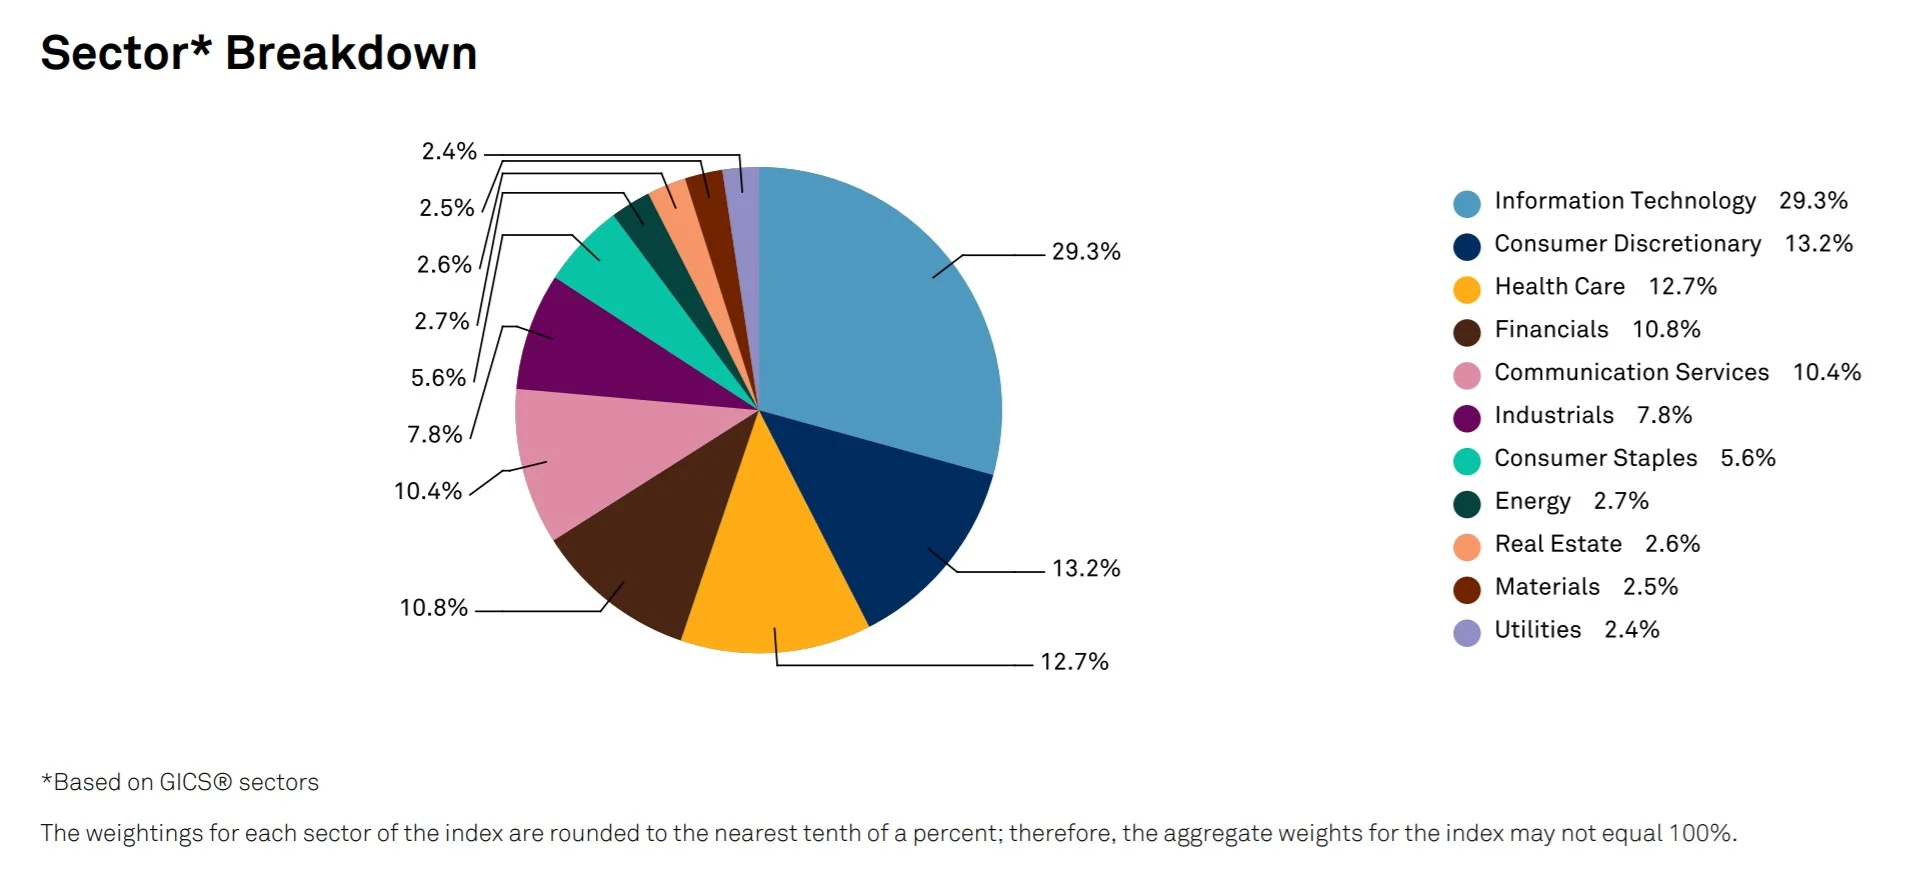
\includegraphics[width=0.6\textwidth]{figures/Sector-SP.png}
    \caption{S\&P 500 Sector Weightings}
    \label{fig:sector_sp}
\end{figure}

\paragraph{Stock Market Sectors}
The rationale behind this selection is multi-staged. Firstly, by including stocks from these predominant sectors, the portfolio captures the performance dynamics of the key drivers of the U.S. equity market. This approach ensures that the portfolio is both diversified and representative of broader market movements. Diversification across different sectors helps mitigate unsystematic risk associated with individual industries or companies, allowing the portfolio to benefit from growth opportunities while reducing the impact of sector-specific downturns.

Secondly, focusing on sectors that contribute most significantly to the S\&P 500 enhances the relevance of the study's findings to investors who benchmark their performance against this widely recognized index. The Information Technology sector, for example, encompasses leading companies in innovation and technology, significantly influencing market trends. The Health Care sector includes firms pivotal in advancing medical technology and pharmaceuticals, demonstrating resilience in various economic conditions.

Industrials and Consumer Discretionary sectors represent core components of the economy, reflecting business cycles and consumer spending patterns, respectively. The Financials sector plays a critical role in economic infrastructure, encompassing banking, insurance, and investment services. By selecting assets from these sectors, the portfolio encompasses areas crucial to economic growth and market capitalization.

This strategic selection aligns with the study's objective of developing a predictive portfolio optimization framework applicable to a realistic and impactful set of assets. It allows for testing the effectiveness of the proposed models and strategies in a context that is meaningful to investors and relevant to overall market performance. Moreover, by focusing on sectors that significantly influence the S\&P 500, the study ensures that its results have practical implications for portfolio management and investment decision-making.

\paragraph{Entropy Methods for Time Series Analysis}
To assess the complexity of the time-series data for these assets, we utilized entropy-based methods. Specifically, we employed the \texttt{OrdianlEntropy} package in Python, which provides time-efficient, ordinal pattern-based entropy algorithms for computing the complexity of one-dimensional time-series. This analysis informed our feature engineering process by highlighting the inherent unpredictability and dynamic behavior of the asset prices.

\subparagraph{Permutation Entropy (PE)}
Permutation Entropy (PE), introduced by Bandt and Pompe in 2002, is a measure of complexity that quantifies the diversity of ordinal patterns in a time series. It is based on the relative ordering of the values within embedding vectors derived from the time series.
Given a time series ${ x_t }_{t=1}^N$, the calculation of PE involves the following steps:

\begin{enumerate} \item \textbf{Embedding the Time Series:}
Choose an embedding dimension $m$ and time delay $\tau$, and construct embedding vectors:
\begin{equation}
    s_i = \left( x_i, x_{i+\tau}, x_{i+2\tau}, \dots, x_{i+(m-1)\tau} \right), \quad i = 1,2,\dots, N - (m -1)\tau.
\end{equation}

\item \textbf{Forming Ordinal Patterns:}

For each embedding vector $s_i$, determine the permutation $\pi_i$ that sorts its components in ascending order:
\begin{equation}
    s_i \rightarrow \left( x_{i+\tau(k_0)} \leq x_{i+\tau(k_1)} \leq \dots \leq x_{i+\tau(k_{m-1})} \right),
\end{equation}
where $(k_0, k_1, \dots, k_{m-1})$ represents the indices of the sorted components.

\item \textbf{Calculating Probabilities:}

Count the frequency of each of the $m!$ possible ordinal patterns $\pi_j$, and estimate their probabilities:
\begin{equation}
    p(\pi_j) = \frac{\text{Number of times pattern } \pi_j \text{ occurs}}{N - (m -1)\tau}.
\end{equation}

\item \textbf{Calculating Permutation Entropy:}

Compute the permutation entropy using Shannon's entropy formula:
\begin{equation}
    \mathrm{PE} = - \sum_{j=1}^{m!} p(\pi_j) \ln p(\pi_j).
\end{equation}

Normalize \ac{PE} by dividing by $\ln(m!)$ to ensure it ranges between 0 and 1:
\begin{equation}
    \mathrm{PE}_{\text{norm}} = \frac{\mathrm{PE}}{\ln(m!)}.
\end{equation}
\end{enumerate}

\begin{itemize} \item A \textbf{low PE} value indicates that the time series has a predictable or regular structure, with fewer unique ordinal patterns. \item A \textbf{high PE} value suggests that the time series is more complex or random, exhibiting a higher diversity of ordinal patterns. \end{itemize}


\subparagraph{Weighted Permutation Entropy (WPE)}
Weighted Permutation Entropy (WPE) enhances PE by incorporating the amplitude information of the time series. It assigns weights to ordinal patterns based on the values within the embedding vectors, thus accounting for both the order and magnitude of the data.
The calculation of \ac{WPE} involves the following steps:

\begin{enumerate} \item \textbf{Embedding and Ordinal Patterns:}
Follow steps 1 and 2 as in the calculation of PE to obtain the embedding vectors and their corresponding ordinal patterns.

\item \textbf{Assigning Weights:}

For each embedding vector $s_i$, calculate a weight $w_i$ based on the amplitude of its components. A common choice is the variance or absolute differences:
\begin{equation}
    w_i = \operatorname{Var}(s_i) = \frac{1}{m} \sum_{k=0}^{m-1} \left( x_{i+\tau k} - \bar{x}_i \right)^2,
\end{equation}
where $\bar{x}_i$ is the mean of the components of $s_i$.

\item \textbf{Calculating Weighted Probabilities:}

For each ordinal pattern $\pi_j$, compute the weighted probability:
\begin{equation}
    p_w(\pi_j) = \frac{\sum_{s_i \in \pi_j} w_i}{\sum_{i=1}^{N - (m -1)\tau} w_i}.
\end{equation}

\item \textbf{Calculating Weighted Permutation Entropy:}

Compute \ac{WPE} using the weighted probabilities:
\begin{equation}
    \mathrm{WPE} = - \sum_{j=1}^{m!} p_w(\pi_j) \ln p_w(\pi_j).
\end{equation}

Normalize WPE similarly to PE:
\begin{equation}
    \mathrm{WPE}_{\text{norm}} = \frac{\mathrm{WPE}}{\ln(m!)}.
\end{equation}
\end{enumerate}
\begin{itemize} \item \textbf{WPE} reflects both the diversity of ordinal patterns and the magnitude of fluctuations in the time series. \item It is more sensitive to significant changes in amplitude, making it useful for detecting volatility and abrupt transitions. \end{itemize}

\subparagraph{Dispersion Entropy (DE)}
Dispersion Entropy (DE), introduced by Rostaghi and Azami in 2016, is an entropy measure that accounts for both the ordering and dispersion of data by mapping the time series into a sequence of classes or symbols.
To calculate DE, follow these steps:

\begin{enumerate} \item \textbf{Mapping Data to Classes:}
Define $c$ classes and map each data point $x_t$ to a class label $k_t$ using a mapping function, such as:
\begin{equation}
    k_t = \left\lfloor c \cdot \frac{x_t - x_{\min} + \epsilon}{x_{\max} - x_{\min} + 2\epsilon} \right\rfloor + 1, \quad k_t \in \{1, 2, \dots, c\},
\end{equation}
where $x_{\min}$ and $x_{\max}$ are the minimum and maximum values of the time series, and $\epsilon$ is a small constant to prevent division by zero.

\item \textbf{Embedding:}

Form embedding vectors of class labels:
\begin{equation}
    s_i = \left( k_i, k_{i+\tau}, k_{i+2\tau}, \dots, k_{i+(m-1)\tau} \right).
\end{equation}

\item \textbf{Creating Dispersion Patterns:}

Each embedding vector $s_i$ represents a dispersion pattern $d_j$, where $j$ indexes the possible patterns.

\item \textbf{Calculating Probabilities:}

Count the frequency of each possible dispersion pattern and estimate their probabilities:
\begin{equation}
    p(d_j) = \frac{\text{Number of times pattern } d_j \text{ occurs}}{N - (m -1)\tau}.
\end{equation}

\item \textbf{Calculating Dispersion Entropy:}

Compute DE using:
\begin{equation}
    \mathrm{DE} = - \sum_{j=1}^{c^m} p(d_j) \ln p(d_j).
\end{equation}

Normalize DE by dividing by $\ln(c^m)$:
\begin{equation}
    \mathrm{DE}_{\text{norm}} = \frac{\mathrm{DE}}{\ln(c^m)}.
\end{equation}
\end{enumerate}

\begin{itemize} \item \textbf{DE} considers both the frequency and dispersion of data, providing a robust measure of complexity for non-stationary time series. \item It effectively captures changes in amplitude and is less sensitive to noise and outliers. \end{itemize}

\subparagraph{Choosing WPE and DE for Stock Price Analysis}
Analyzing stock prices requires accounting for both the order and magnitude of price changes due to the following reasons:

\subparagraph{Advantages of WPE}

Weighted Permutation Entropy (WPE) offers distinct benefits in the analysis of financial time series by effectively incorporating the amplitude of price changes into its computation. By weighting ordinal patterns, WPE not only captures the direction of changes but also accounts for their magnitude, making it particularly adept at identifying periods of heightened market volatility. This sensitivity to volatility is crucial for risk management, as it allows analysts to detect significant shifts in market behavior that could impact investment decisions. Furthermore, WPE strikes a balance between computational efficiency and analytical depth. It provides detailed insights into the complexity of financial data without requiring excessive computational resources, making it a practical tool for real-time and large-scale applications.


\subparagraph{Advantages of DE}

Dispersion Entropy (DE) excels in handling the complexities of non-stationary financial time series, which often exhibit trends, abrupt changes, and varying volatility. By mapping data into discrete classes, DE adapts effectively to non-stationarity, ensuring robust analysis across different market conditions. Its design also makes it less sensitive to noise and outliers, a significant advantage in the inherently noisy financial domain, where anomalies can skew traditional measures. DE provides a comprehensive view of market dynamics by considering both the frequency and amplitude of patterns, capturing subtle shifts in market behavior.

Another notable advantage of DE is its amplitude sensitivity. In financial markets, the size of price movements has a direct impact on returns and risks, and methods like DE that incorporate this information provide a richer understanding of market dynamics. Additionally, DE is particularly effective at detecting varying levels of volatility, which play a critical role in shaping investment strategies. Its ability to seamlessly handle the non-stationarity of stock prices, which often undergo regime changes and unpredictable trends, further solidifies its value in financial analysis.

Both WPE and DE offer robust tools for analyzing financial markets, with WPE emphasizing computational balance and volatility capture, while DE focuses on non-stationarity adaptation and comprehensive market understanding. Together, they provide complementary approaches to understanding the complexity of financial time series.
\subparagraph{Conclusion}
Weighted Permutation Entropy (WPE) and Dispersion Entropy (DE) prove to be superior tools compared to traditional Permutation Entropy when analyzing stock prices. These methods capture essential information about both the direction and magnitude of price movements, offering a more nuanced understanding of financial time-series data. Their ability to handle the inherent non-stationarity and volatility of financial markets makes them particularly well-suited for detecting patterns and trends that are often overlooked by simpler measures. Furthermore, WPE and DE provide more informative and sensitive complexity measures, enabling analysts to enhance asset selection and refine risk assessment strategies.

By utilizing \ac{WPE} and \ac{DE}, analysts and investors can achieve a deeper understanding of market behavior, uncovering the complexity and predictability of stock prices. These insights facilitate more informed decisions in selecting assets across different sectors, ultimately improving portfolio management and investment outcomes.
\subsection{Data Sources and Time Period}


To acquire the historical market data necessary for this study, we employed the EOD Historical Data API, a reputable and comprehensive source for end-of-day and historical financial data across various asset classes. The data retrieval process was automated using a Python script that constructs API requests based on the asset ticker, desired data period (e.g., daily, weekly), and specified date range.

For U.S.-listed assets, the script utilizes the endpoint format:

\begin{verbatim}
https://eodhd.com/api/eod/{ticker}.US?period={period}&api_token={api_token}
\end{verbatim}

where \texttt{\{ticker\}} represents the stock symbol, \texttt{\{period\}} denotes the data frequency, \texttt{\{api\_token\}} is the authentication token, and \texttt{\{start\_date\}} and \texttt{\{end\_date\}} define the data range. For Bitcoin (BTC), which is categorized differently in the API, the script accesses data using the endpoint:

\begin{verbatim}
https://eodhd.com/api/eod/BTC-USD.CC?period={period}&api_token={api_token}
\end{verbatim}

An API token, securely stored using environment variables to maintain confidentiality, is included in the requests for authentication. The script handles HTTP responses by checking for successful status codes and raising exceptions in case of errors, ensuring robust data retrieval.

Upon receiving a valid response, the JSON data is parsed into a pandas DataFrame for efficient data manipulation and analysis. The DataFrame includes essential financial indicators such as open, high, low, close prices, and trading volumes. The data is then saved as a CSV file in a structured directory hierarchy corresponding to each asset, following the path:

\begin{verbatim}
../Stocks/{ticker}/{ticker}_us_{period}.csv
\end{verbatim}

By automating the data fetching and saving process, we ensured consistency and repeatability in data collection of the whole pipeline. 
This method allowed us to systematically gather historical market data for all selected assets over the specified time periods, providing a reliable dataset for training the Gaussian Process Regression models and conducting backtesting for the portfolio optimization strategies. 
The use of the EOD Historical Data API ensured that the data was up-to-date and accurate, reflecting real market conditions essential for the validity of our analysis.
Also, for future work, the script can be easily adapted to retrieve data for additional assets or extend the time period, enabling further research and analysis in the financial domain.

\subsection{Data Preprocessing and Log Returns}
Data preprocessing and feature engineering are critical steps in preparing the dataset for modeling. They ensure that the data fed into the Gaussian Process Regression models are clean, consistent, and informative.

\paragraph{Use of Log Returns}

In this project, log returns are utilized for modeling asset price movements due to several compelling reasons that align with both theoretical and practical considerations in financial analysis.

\subparagraph{Theoretical Foundation in Finance}

Log returns are integral to many foundational financial models, such as the Black-Scholes option pricing model, which assume that asset prices follow a log-normal distribution. By using log returns, we align our modeling approach with these theoretical frameworks, facilitating more accurate and consistent analyses. \ac{GPR} models assume normally distributed outputs, and since log returns of log-normally distributed prices are normally distributed, this compatibility enhances the effectiveness of our predictive modeling.

\subparagraph{Stability Over Time}

Log returns exhibit greater stability compared to simple arithmetic returns, particularly in the presence of extreme outliers or during periods of high market volatility. They tend to smooth out spikes and reduce the impact of short-term noise, making the models less sensitive to sudden market anomalies. This stability is crucial for developing robust predictive models that can perform reliably under various market conditions.

\subparagraph{Time Consistency (Additivity)}

One of the key mathematical properties of log returns is their additive nature over time. The total log return over a period is the sum of the log returns over sub-periods:

\begin{equation}
\log\left( \frac{S_t}{S_0} \right) = \log\left( \frac{S_t}{S_{t-1}} \right) + \log\left( \frac{S_{t-1}}{S_{t-2}} \right) + \dots + \log\left( \frac{S_1}{S_0} \right),
\end{equation}

where $S_t$ is the asset price at time $t$. This additive property simplifies the computation of returns over arbitrary time horizons, such as weekly or monthly periods, by allowing us to sum daily log returns. It is particularly beneficial for forecasting and portfolio optimization over multi-day horizons, as it facilitates the aggregation of returns without the need for complex compounding calculations.

\subparagraph{Normalization of Price Scale}

Log returns are scale-invariant, meaning they standardize returns across assets regardless of their price levels. Whether an asset is priced at \$1 or \$1,000, the log return brings their percentage changes onto a consistent scale. This normalization simplifies comparisons across assets with vastly different price levels and reduces the need for additional data scaling or normalization procedures. It ensures that no single asset disproportionately influences the model due to its absolute price, allowing for a more balanced and equitable analysis within the portfolio.

\subparagraph{Conclusion}

By incorporating log returns into our modeling framework, we leverage their theoretical compatibility with financial models, enhance stability against market volatility, benefit from their time-additive properties, and achieve scale normalization across diverse assets. These advantages contribute to the robustness and accuracy of our Gaussian Process Regression models and improve the effectiveness of our dynamic portfolio optimization strategies.



\paragraph{Data Normalization and Scaling}

To bring all features onto a similar scale and improve the numerical stability of the models, we applied data normalization techniques. Specifically, we used min-max scaling to normalize the historical return features and the time index:

\begin{equation}
    X_{\text{normalized}} = \frac{X - X_{\text{min}}}{X_{\text{max}} - X_{\text{min}}},
\end{equation}

where $X$ represents the original feature values, and $X_{\text{min}}$ and $X_{\text{max}}$ are the minimum and maximum values of the feature, respectively. This scaling transforms the data to a [0, 1] range, facilitating efficient model training.

\paragraph{Treatment of Missing Data and Outliers}

Financial time-series data often contain missing values and outliers due to market closures, data recording errors, or extreme market events. To address missing data, we employed interpolation methods appropriate for time-series, such as linear interpolation and forward/backward filling, ensuring temporal continuity in the data.

Outliers were identified using the Interquartile Range (IQR) method:

\begin{equation}
    \text{IQR} = Q_3 - Q_1,
\end{equation}

where $Q_1$ and $Q_3$ are the first and third quartiles, respectively. Data points lying outside 1.5 times the IQR from the quartiles were considered outliers. We assessed these outliers to determine whether they were due to data errors or genuine market anomalies. Genuine outliers representing significant market movements were retained to preserve the dataset's integrity, while erroneous data points were corrected or removed.

\paragraph{Handling Missing Data with GPR}
\ac{GPR} is particularly effective in addressing missing data and managing outliers due to its probabilistic framework and ability to model uncertainties. As demonstrated in the figure, GPR leverages the observed data points to predict missing values by constructing a distribution over possible functions that fit the data. 
As shown in \ref{fig:gpr_missing_outliers} for each prediction, GPR provides both a mean estimate and a confidence interval that quantifies the uncertainty of the prediction. This feature allows it to interpolate missing data seamlessly while considering the underlying patterns and relationships in the time-series.

\begin{figure}[htbp]
    \centering
    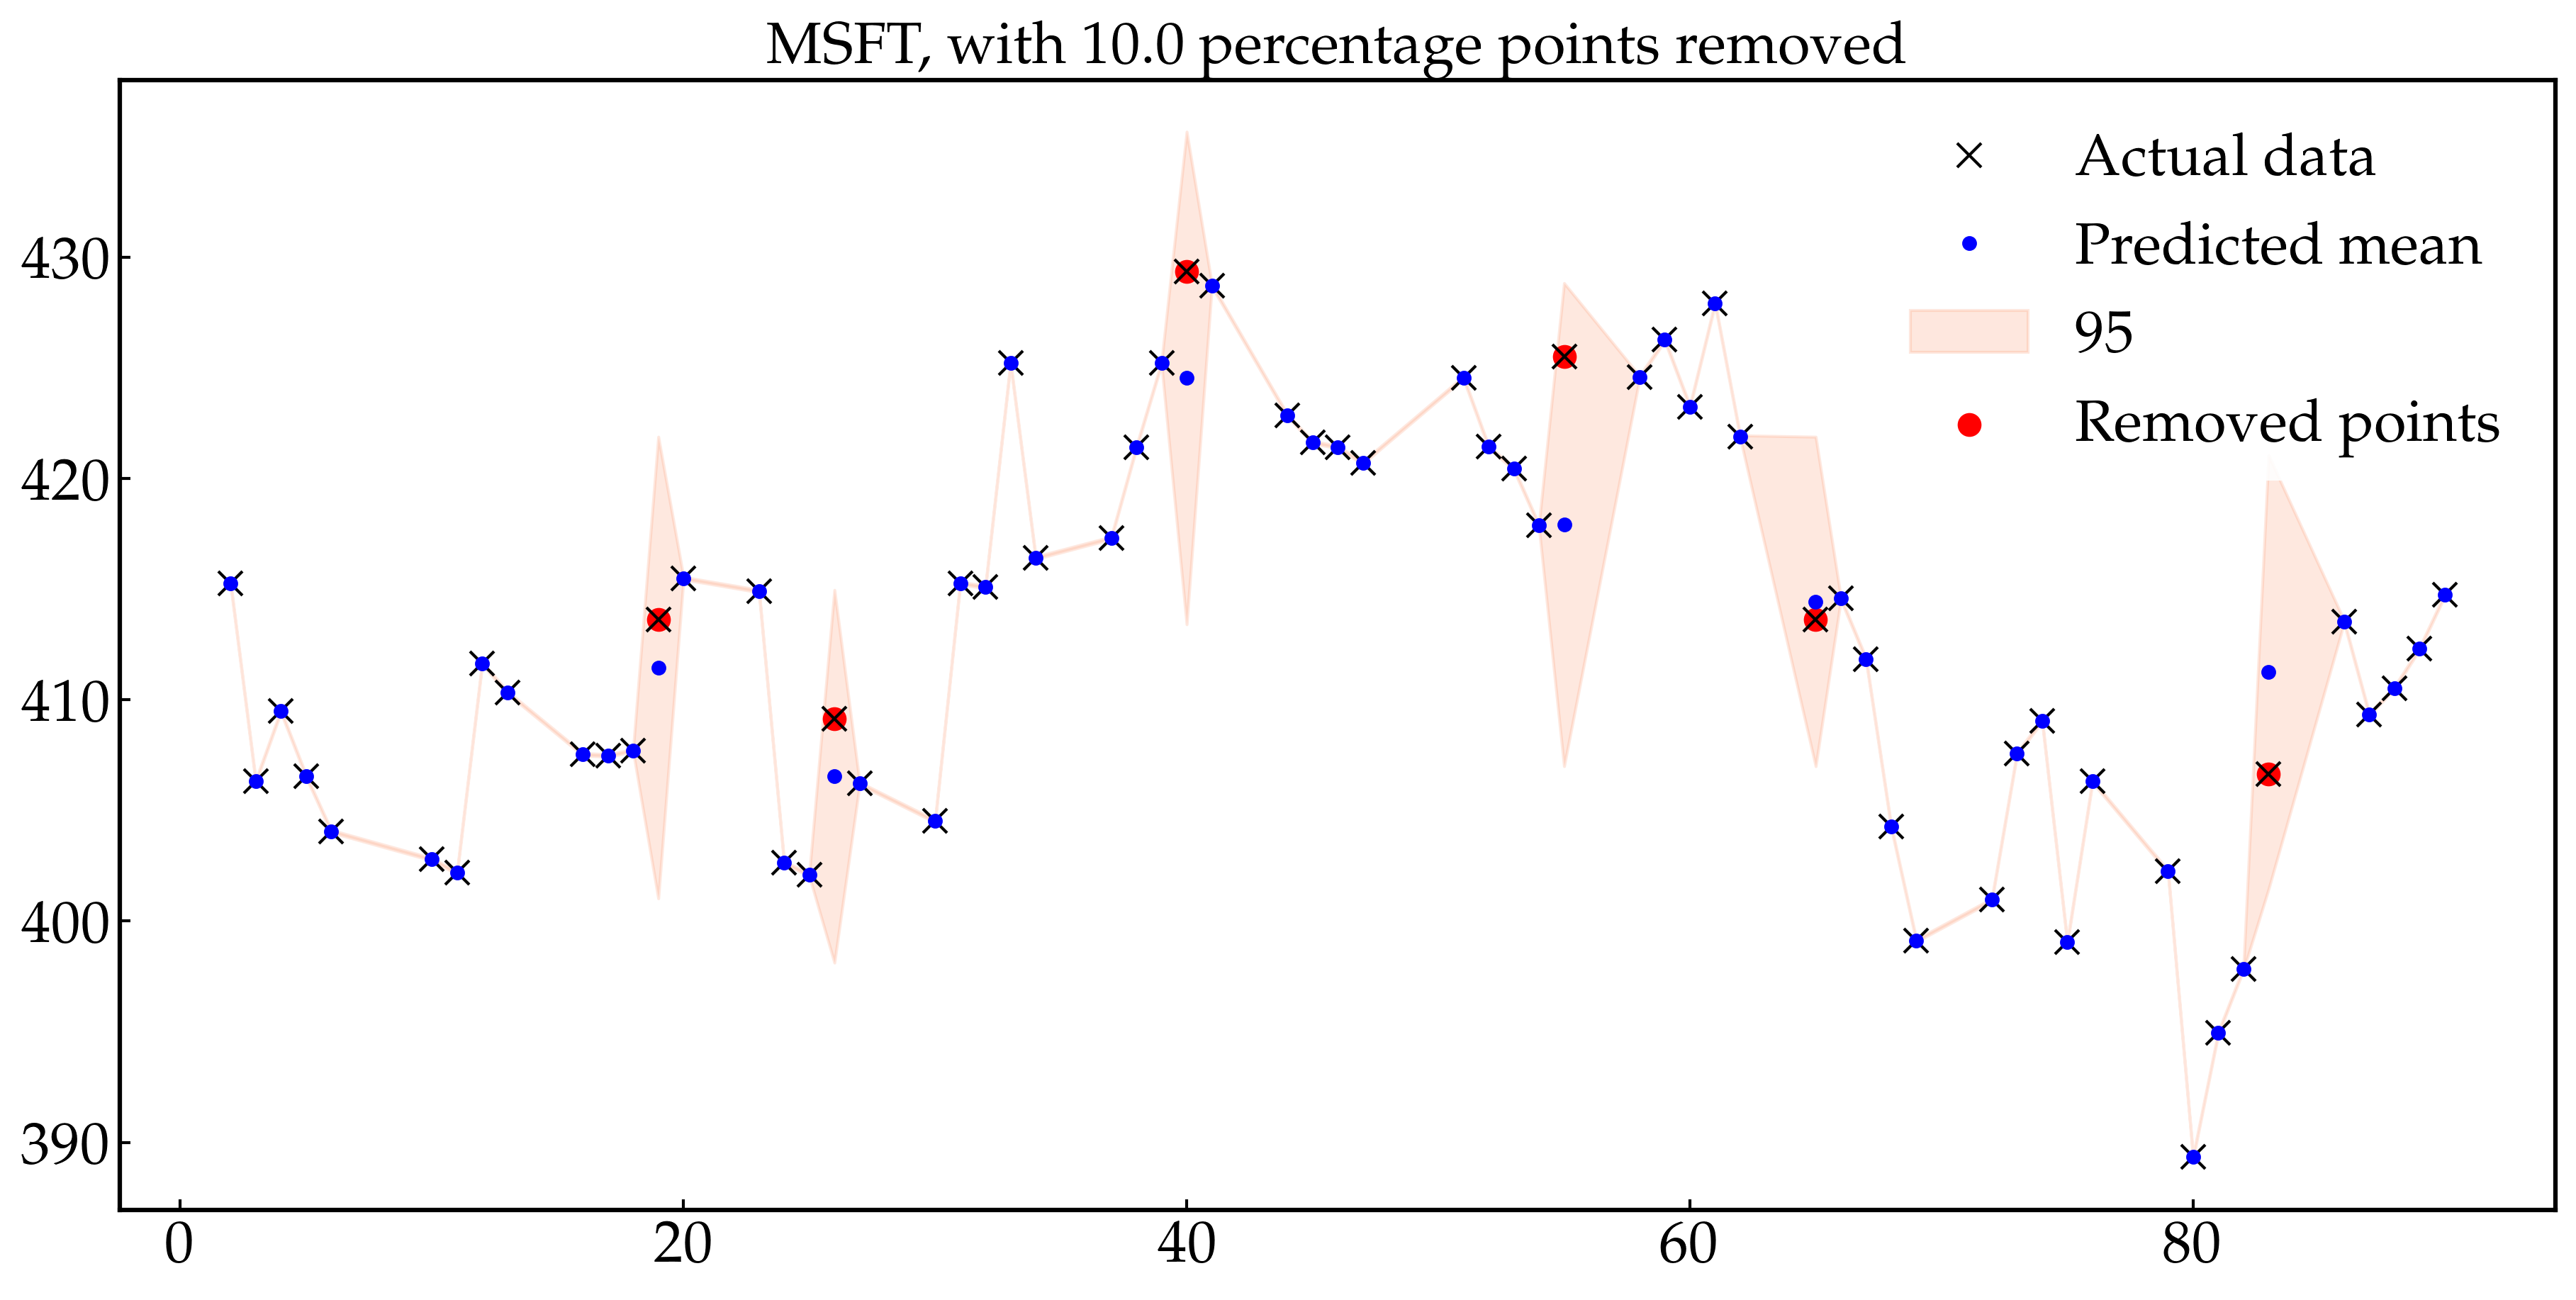
\includegraphics[width=0.6\textwidth]{figures/predicted_MSFT_with_removed.png}
    \caption{GPR Prediction with Missing Data and Outliers}
    \label{fig:gpr_missing_outliers}
\end{figure}

Furthermore, GPR handles outliers by naturally weighting data points according to their fit within the modeled distribution. Outliers, which deviate significantly from the predicted mean and exhibit higher uncertainty, are less influential in the model's predictions. This property prevents extreme values from distorting the regression output, making GPR robust in noisy and incomplete datasets. The ability to quantify uncertainty not only aids in filling missing data but also provides a valuable tool for identifying potential anomalies in the dataset, as seen in the highlighted regions of the plot. By incorporating these capabilities, GPR ensures that the dataset remains coherent and usable for subsequent analysis, such as predictive modeling and portfolio optimization.


\paragraph{Data Splitting and Cross-Validation}

The dataset was divided into training and testing sets to evaluate the model's predictive performance. The training set consisted of the first 80\% of the time period, while the remaining 20\% was reserved for testing. This chronological split respects the temporal order of the data, avoiding look-ahead bias.

To further validate the models, we used time-series cross-validation with a rolling window approach. In each iteration, the model was trained on a window of consecutive data points and tested on the subsequent period. This method provides a more robust assessment of the model's performance over time and simulates real-world forecasting conditions.

\paragraph{Sliding Window Approach}

To denoise the time-series data and reduce short-term fluctuations, we employed a sliding window approach using a centered rolling window mechanism. For each data point in the series, a window of a specified size $w$ was centered around it, and a statistical function was applied to the data within this window to compute a denoised value. The primary function used was the mean, though other functions could be applied as needed.

Formally, let $\{ x_t \}_{t=1}^T$ represent the original time-series data, and $\{ \tilde{x}_t \}_{t=1}^T$ denote the denoised series. The denoised value at time $t$, $\tilde{x}_t$, is calculated as:

\begin{equation}
\tilde{x}_t = \frac{1}{n_t} \sum_{i = t - k}^{t + k} x_i,
\end{equation}

where $k = \left\lfloor \frac{w}{2} \right\rfloor$, and $n_t$ is the number of data points within the window centered at time $t$. The window size $w$ is an odd integer to ensure symmetry around the central point. At the edges of the time-series (when $t - k < 1$ or $t + k > T$), the window is adjusted by including available data points, and the minimum number of periods is set to 1 to allow computation even with incomplete windows.

To handle any missing values that may arise at the edges due to insufficient data points, we applied forward and backward filling methods. Forward filling propagates the last observed non-missing value forward to fill subsequent missing positions, while backward filling fills missing values by propagating the next observed non-missing value backward. These steps ensure that the denoised series is complete and free from missing values.

This sliding window denoising process effectively smooths the data by averaging over the local neighborhood of each data point, reducing random noise while preserving significant trends and patterns. By enhancing the signal-to-noise ratio in the time-series, this approach improves the quality of the input data for the Gaussian Process Regression models, leading to better predictive performance and more reliable portfolio optimization decisions.

\paragraph{Gaussian Filter Denoising Method}

To further enhance the quality of the time-series data and reduce high-frequency noise, we employed the Gaussian filter denoising method. The Gaussian filter is a convolutional filter that applies a Gaussian kernel to smooth data by averaging neighboring points with weights determined by the Gaussian function. This technique preserves significant trends and patterns while effectively attenuating random fluctuations and noise.

The Gaussian kernel is defined by the Gaussian (normal) distribution function:

\begin{equation}
G(i) = \frac{1}{\sqrt{2\pi} \sigma} \exp\left( -\frac{i^2}{2\sigma^2} \right),
\end{equation}

where $i$ is the index distance from the central data point, and $\sigma$ is the standard deviation of the Gaussian distribution, controlling the degree of smoothing. A larger $\sigma$ results in a wider kernel and more extensive smoothing.

The denoised value at time $t$, $\tilde{x}_t$, is computed by convolving the original time-series data $x_t$ with the Gaussian kernel:

\begin{equation}
\tilde{x}_t = \sum_{i = -k}^{k} G(i) \cdot x_{t + i},
\end{equation}

where $k$ is the window size parameter determining the range of data points considered around time $t$.

In our implementation, we applied the Gaussian filter to the closing prices of the assets using a standard deviation $\sigma = 1$, which provides a balanced smoothing effect without overly distorting the data. The following code snippet illustrates the application of the Gaussian filter using the \texttt{gaussian\_filter} function from the SciPy library in Python:

\begin{lstlisting}[language=Python]
if isFiltered:
    df['filtered_close'] = gaussian_filter(df['close'], sigma=1)
\end{lstlisting}

In this code, \texttt{df['close']} represents the original closing price data, and \texttt{df['filtered\_close']} stores the denoised data after applying the Gaussian filter. The \texttt{isFiltered} flag allows for conditional application of the filtering process.

By using the Gaussian filter denoising method, we effectively reduced the impact of noise and short-term fluctuations in the financial time-series data. This preprocessing step enhances the signal-to-noise ratio, allowing the Gaussian Process Regression models to focus on underlying market trends and improving the accuracy of the return predictions. The combination of the sliding window approach and Gaussian filtering provides a robust methodology for data smoothing, contributing significantly to the reliability and performance of the predictive modeling and subsequent portfolio optimization.

The filtered data retained essential market movements while reducing random fluctuations, allowing the Gaussian Process Regression models to focus on meaningful signals.


\subsection{Summary}

By carefully selecting assets, sourcing reliable data, and meticulously preprocessing the dataset, we established a solid foundation for our predictive modeling. The combination of normalization, outlier treatment, strategic data splitting, and denoising ensured that the inputs to our models were of high quality. These steps are crucial for enhancing the performance of the Gaussian Process Regression models and, ultimately, for developing effective portfolio optimization strategies.



\section{Model Development}
In this section, we outline the development of the predictive framework and evaluation methodology for forecasting asset returns and optimizing portfolio allocations, namely trading strategies. The focus is on the performance metrics used to assess model effectiveness, as well as the selection of a baseline model for comparison with the Gaussian Process Regression (GPR) approach.

\subsection{Baseline Models}

To establish a reference point for the performance of the Gaussian Process Regression model, we selected the ARIMA (AutoRegressive Integrated Moving Average) model as the baseline.

\subsubsection{\ac{ARIMA} Model}

The \ac{ARIMA} model is a widely used time-series forecasting technique that combines autoregressive (AR), differencing (I), and moving average (MA) components. It is defined by three parameters: $p$, $d$, and $q$, where:

\begin{itemize}
    \item $p$ is the order of the autoregressive term.
    \item $d$ is the degree of differencing required to achieve stationarity.
    \item $q$ is the order of the moving average term.
\end{itemize}

The \ac{ARIMA} model forecasts the value at time $t$ as:

\begin{equation}
y_t = \phi_1 y_{t-1} + \phi_2 y_{t-2} + \dots + \phi_p y_{t-p} + \epsilon_t + \theta_1 \epsilon_{t-1} + \dots + \theta_q \epsilon_{t-q},
\end{equation}

where $\phi_i$ are the AR coefficients, $\theta_i$ are the MA coefficients, and $\epsilon_t$ is the white noise term.

\subsubsection{Rationale for Baseline Selection}

The \ac{ARIMA} model serves as an appropriate baseline because it is a well-established method for modeling time-series data and capturing trends and seasonality. While it is linear in nature, ARIMA provides a benchmark for assessing the added value of GPR, which can capture complex non-linear relationships and quantify uncertainty in predictions.

\subsection{Comparative Evaluation}

The performance of the \ac{GPR} model is compared against the \ac{ARIMA} baseline using the \ac{MSE} for predictive accuracy and the Sharpe Ratio for portfolio optimization outcomes. This dual evaluation approach ensures that the models are assessed comprehensively, both in terms of their forecasting ability and their impact on investment decisions. By demonstrating improvements over the \ac{ARIMA} model, the study highlights the effectiveness of \ac{GPR} in dynamic portfolio management.

\subsection{Performance Metrics}

To evaluate the performance of the predictive models and portfolio strategies, we employ the following metrics:

\subsubsection{Mean Squared Error (MSE)}

The Mean Squared Error (MSE) measures the accuracy of the model's predictions compared to the actual observed values. It is calculated as:

\begin{equation}
\text{MSE} = \frac{1}{n} \sum_{i=1}^{n} \left( y_i - \hat{y}_i \right)^2,
\end{equation}

where $y_i$ represents the actual value, $\hat{y}_i$ is the predicted value, and $n$ is the total number of predictions. A lower MSE indicates better predictive accuracy. This metric is particularly useful for evaluating the performance of GPR and baseline models in forecasting asset returns.

\subsubsection{Sharpe Ratio}

The Sharpe Ratio assesses the risk-adjusted performance of a portfolio, measuring the excess return per unit of risk. It is defined as:

\begin{equation}
\text{Sharpe Ratio} = \frac{E[R_p] - R_f}{\sigma_p},
\end{equation}

where $E[R_p]$ is the expected portfolio return, $R_f$ is the risk-free rate, and $\sigma_p$ is the portfolio's standard deviation of returns. A higher Sharpe Ratio indicates a more favorable trade-off between risk and return, making it a crucial metric for evaluating the effectiveness of the portfolio optimization strategies derived from the predicted returns.

\subsection{Multi-Input Gaussian Process Regression Model}

In this study, we developed a multi-input Gaussian Process Regression (GPR) model that incorporates multiple economic factors and time as input dimensions to predict the returns of individual stocks. The model combines features from a diverse set of assets and economic indicators, including Brent Oil prices, the US Dollar Index (DXY), the S\&P 500 Index, the Nasdaq 100 Index, Bitcoin (BTC), and gold prices (XAU/USD). This multi-input framework allows the model to capture intricate relationships between the target stock and broader market dynamics, enhancing its predictive power.

\subsubsection{Input Data and Feature Selection}

The input features for the GPR model were selected based on their correlation with the target stock. For each feature, we calculated the correlation between the feature's historical returns and the target stock's returns. Only features with an absolute correlation exceeding a predefined threshold were included in the model to ensure relevance and reduce noise in the predictions. This approach prioritizes the most influential economic factors while discarding irrelevant or weakly correlated inputs.

The final input matrix was constructed by concatenating the selected features along with time as an additional dimension. By including time, the model accounts for temporal trends and seasonality in the data, further improving its predictive capabilities.

\subsubsection{Composite Kernel for Multi-Dimensional Inputs}

To effectively model the multi-dimensional input space, we employed a composite kernel approach that assigns separate kernels to different input dimensions. Specifically:

\begin{itemize}
    \item One kernel was applied to the economic factors, allowing the model to learn the specific relationships between the target stock and each factor. This kernel captures the varying scales and complexities of the economic data.
    \item Another kernel was applied to the time dimension, enabling the model to account for temporal dependencies and trends. 
\end{itemize}

The composite kernel combines these two components multiplicatively, ensuring that the model can flexibly adjust to different input dimensions and set appropriate length scales for each. This design allows the GPR model to capture the unique characteristics of each feature while modeling their joint effects on the target stock's returns.

\subsubsection{Training and Testing Framework}

The training and testing process involved splitting the data into separate periods. The training set included data from the beginning of the time series up to a specified date, while the testing set encompassed the subsequent period. This split ensured that the model was evaluated on unseen data, simulating real-world forecasting conditions.

To further enhance the model's robustness, the noise variance in the GPR model was either fixed to a small value or optimized as a trainable parameter. This dual approach ensured flexibility in handling data with varying noise levels while preventing overfitting.

\subsubsection{Prediction and Evaluation}

Once the model was trained, it was used to predict the returns of the target stock over the testing period. The predictive mean and variance were computed for each test point, providing both point estimates and uncertainty bounds. The model's performance was evaluated using the Mean Squared Error (MSE), calculated for both normalized and denormalized data, to assess its accuracy in both relative and absolute terms.

By leveraging multi-input GPR with composite kernels, this approach captures the interplay between diverse economic factors, time, and stock returns. The flexibility in kernel design and inclusion of multi-dimensional inputs ensures that the model is both robust and adaptive, providing accurate predictions for individual stock performance in dynamic market environments.

\subsection{Hyperparameter Tuning}

Effective hyperparameter tuning is crucial for optimizing the performance of \ac{GPR} models, as it directly impacts the model's ability to fit the data and generalize to unseen samples. In this study, two distinct approaches were implemented for training \ac{GPR} models, differing in how the likelihood variance (noise variance) was treated during the optimization process. This subsection describes the methodologies and their respective advantages.

\subsubsection{Fixed Likelihood Variance}

In the first approach, the likelihood variance was fixed to a predefined value ($\sigma^2 = 10^{-3}$) and excluded from the training process. By keeping the noise variance constant, the optimization focuses solely on tuning the parameters of the kernel function, ensuring that the model does not overfit to noise in the data. This approach is computationally efficient and is particularly useful when the level of noise in the data is well-understood or consistent across the dataset. The training process involved minimizing the model's negative log marginal likelihood using the Scipy optimizer provided by \texttt{gpflow}:

\begin{equation}
\text{Negative Log Marginal Likelihood (NLML)} = -\log p(\mathbf{y} | \mathbf{X}, \boldsymbol{\theta}),
\end{equation}

where $\boldsymbol{\theta}$ represents the trainable kernel parameters.

\subsubsection{Trainable Likelihood Variance}

In the second approach, the likelihood variance was set as a trainable parameter, allowing the model to adaptively learn the optimal noise level from the data. This method is advantageous when the data contains varying levels of noise or when the noise characteristics are not well-understood. To enhance the robustness of this approach, multiple starting values for the likelihood variance were used ($10^{-5}$, $10^{-3}$, $10^{-1}$, $1.0$), ensuring that the optimization process explored a diverse range of initial configurations. For each starting variance, the model was trained using the Scipy optimizer, and the final negative log marginal likelihood was evaluated.

\begin{itemize}
    \item The model with the lowest final loss was selected as the best-performing model.
    \item This approach balances the trade-off between model flexibility and the risk of overfitting by optimizing both the kernel parameters and the likelihood variance.
\end{itemize}

\subsubsection{Comparison of Approaches}

Both approaches were evaluated based on their ability to minimize the negative log marginal likelihood and the predictive performance on the test dataset. The fixed likelihood variance method provided computational simplicity and reduced the risk of overfitting in scenarios with stable noise levels. Conversely, the trainable likelihood variance approach demonstrated higher adaptability, allowing the model to account for varying noise levels and capture the data's inherent uncertainty more effectively.

\subsubsection{Best Model Selection}

The trainable likelihood variance approach, with multiple initializations, identified the model configuration that minimized the negative log marginal likelihood. This model provided a balance between accurately capturing the signal and accounting for noise, making it the preferred choice for the Gaussian Process Regression framework used in this study.


\section{Forecasting Approach}
Describe the iterative forecasting method and how predictions are updated daily.

\subsection{Iterative Retraining for Sequential Predictions}

In addition to batch training and prediction, we implemented an iterative retraining approach for the Gaussian Process Regression (GPR) model. This method reflects a real-world scenario where new market data becomes available daily, requiring the model to be updated frequently to make accurate short-term predictions. In this approach, the GPR model is retrained daily using all available data up to the current day, and predictions are made for the next day. This process is repeated iteratively for five consecutive days to generate predictions for a five-day horizon.

\subsubsection{Methodology}

The iterative retraining approach involves the following steps:

\begin{enumerate}
    \item \textbf{Daily Data Integration:} At the start of each iteration, the most recent daily market data is fetched and added to the training dataset. This includes the latest values of the target stock and selected economic factors.
    \item \textbf{Training with Updated Data:} The GPR model is retrained using the expanded dataset, incorporating all historical data up to the current day. Both fixed and trainable likelihood variance configurations are evaluated to ensure robust performance.
    \item \textbf{Prediction for the Next Day:} Using the retrained model, predictions are made for the target stock's return for the next day. The predictive mean and variance are recorded for each iteration.
    \item \textbf{Iterative Execution:} Steps 1 through 3 are repeated iteratively, with each new day’s data being integrated into the model, until predictions are generated for all five future days.
\end{enumerate}

\subsubsection{Advantages of Iterative Retraining}

The iterative retraining approach offers several advantages:

\begin{itemize}
    \item \textbf{Real-Time Adaptation:} By retraining the model daily, it continuously adapts to the latest market conditions, ensuring that predictions remain relevant and responsive to recent trends.
    \item \textbf{Enhanced Short-Term Accuracy:} The use of updated data allows the model to account for the most recent market dynamics, improving the accuracy of short-term forecasts.
    \item \textbf{Uncertainty Quantification:} With each iteration, the GPR model provides a predictive mean and variance for the next day, enabling the assessment of uncertainty in the predictions. This is particularly useful for risk-aware decision-making in portfolio management.
\end{itemize}

\subsubsection{Performance Evaluation}

To evaluate the effectiveness of this approach, the Mean Squared Error (MSE) was calculated for both normalized and denormalized predicted returns across the five days. The iterative predictions were also compared against actual returns to assess the model's ability to track short-term market movements. Additionally, the cumulative performance over the five-day horizon was analyzed to understand the overall impact of daily updates on predictive accuracy.

\subsubsection{Practical Application}

This iterative retraining approach closely mimics real-world trading scenarios where investors rely on daily market updates to make decisions. By retraining the model with the latest data and predicting only one day ahead, this method ensures that the predictions are both timely and aligned with current market conditions. This sequential prediction framework provides a robust foundation for dynamic portfolio management, enabling more accurate and adaptive asset allocation strategies.



\section{Portfolio Optimization Strategies}

\subsection{Traditional Strategies}
\subsubsection{Maximum Return Strategy Formulation}

The maximum return strategy aims to maximize the expected return of a portfolio while considering risk constraints and incorporating regularization penalties such as L1/L2 norms and transaction costs. The optimization problem is formulated based on the given code snippet and can be expressed mathematically as follows.

Let:

\begin{itemize}
    \item \( \mathbf{w} \in \mathbb{R}^n \) be the vector of portfolio weights for \( n \) assets.
    \item \( \boldsymbol{\mu} \in \mathbb{R}^n \) be the vector of expected returns for each asset.
    \item \( \Sigma \in \mathbb{R}^{n \times n} \) be the covariance matrix of asset returns.
    \item \( \sigma_{\text{max}} \) be the maximum allowable portfolio volatility.
    \item \( \mathcal{R}(\mathbf{w}) \) be the regularization penalty function, which may include L1/L2 penalties and transaction costs.
\end{itemize}

The optimization problem is:

\[
\begin{aligned}
\min_{\mathbf{w}} & \quad -\mathbf{w}^\top \boldsymbol{\mu} + \mathcal{R}(\mathbf{w}) \\
\text{subject to} & \quad \sqrt{\mathbf{w}^\top \Sigma \mathbf{w}} \leq \sigma_{\text{max}} \\
& \quad \sum_{i=1}^n w_i = 1 \\
& \quad w_i \geq 0, \quad \forall i \in \{1, \dots, n\}
\end{aligned}
\]

\paragraph{Objective Function}

The objective function consists of two components:

\begin{enumerate}
    \item \textbf{Negative Expected Return}: \( -\mathbf{w}^\top \boldsymbol{\mu} \)
    \item \textbf{Regularization Penalty}: \( \mathcal{R}(\mathbf{w}) \)
\end{enumerate}

By minimizing the negative expected return, we effectively maximize the portfolio's expected return. The regularization penalty \( \mathcal{R}(\mathbf{w}) \) accounts for additional considerations such as promoting sparsity (L1 regularization), preventing overfitting (L2 regularization), and minimizing transaction costs.

\paragraph{Constraints}

The constraints ensure that:

\begin{itemize}
    \item \textbf{Volatility Constraint}: The portfolio's volatility does not exceed \( \sigma_{\text{max}} \):

    \[
    \sqrt{\mathbf{w}^\top \Sigma \mathbf{w}} \leq \sigma_{\text{max}}
    \]

    \item \textbf{Full Investment Constraint}: The sum of the portfolio weights equals 1:

    \[
    \sum_{i=1}^n w_i = 1
    \]

    \item \textbf{No Short-Selling Constraint}: All portfolio weights are non-negative:

    \[
    w_i \geq 0, \quad \forall i
    \]
\end{itemize}

\paragraph{Regularization Penalty}

The regularization penalty \( \mathcal{R}(\mathbf{w}) \) can be detailed as:

\[
\mathcal{R}(\mathbf{w}) = \lambda_1 \|\mathbf{w}\|_1 + \lambda_2 \|\mathbf{w}\|_2^2 + \gamma \sum_{i=1}^n |w_i - w_i^{\text{prev}}|
\]

where:

\begin{itemize}
    \item \( \|\mathbf{w}\|_1 = \sum_{i=1}^n |w_i| \) is the L1 norm, promoting sparsity in the portfolio weights.
    \item \( \|\mathbf{w}\|_2^2 = \sum_{i=1}^n w_i^2 \) is the squared L2 norm, preventing extreme weight allocations.
    \item \( w_i^{\text{prev}} \) is the previous weight of asset \( i \), accounting for transaction costs when adjusting the portfolio.
    \item \( \lambda_1, \lambda_2, \gamma \geq 0 \) are hyperparameters controlling the influence of each penalty component.
\end{itemize}

\paragraph{Optimization Method}

The optimization problem is solved using the Sequential Least Squares Programming (SLSQP) algorithm, which is suitable for constrained nonlinear optimization. The method minimizes the objective function while satisfying the specified constraints.

\[
\text{Result} = \arg\min_{\mathbf{w}} \left( -\mathbf{w}^\top \boldsymbol{\mu} + \mathcal{R}(\mathbf{w}) \right)
\]

\[
\text{subject to constraints}
\]

\paragraph{Implementation Notes}

In our implementation:

\begin{itemize}
    \item The function \texttt{returns\_objective} computes the objective function.
    \item The \texttt{maximize\_returns} method sets up the optimization problem, including the volatility constraint and any additional constraints.
    \item Regularization and transaction costs are incorporated through the \texttt{total\_penalty} function.
\end{itemize}

By formulating the strategy in this manner, the model seeks the optimal balance between maximizing returns and controlling for risk and costs, resulting in a robust and practical portfolio optimization solution.


\subsubsection{Maximum Sharpe Ratio Optimization}

The maximum Sharpe ratio optimization aims to maximize the portfolio's Sharpe ratio, which is a measure of risk-adjusted return. This involves finding the optimal portfolio weights that maximize the expected return minus the risk-free rate, divided by the portfolio's volatility, while also incorporating regularization penalties such as L1/L2 norms and transaction costs.

Let:

\begin{itemize}
    \item \( \mathbf{w} \in \mathbb{R}^n \) be the vector of portfolio weights for \( n \) assets.
    \item \( \boldsymbol{\mu} \in \mathbb{R}^n \) be the vector of expected returns for each asset.
    \item \( \Sigma \in \mathbb{R}^{n \times n} \) be the covariance matrix of asset returns.
    \item \( r_f \) be the risk-free rate.
    \item \( \mathcal{R}(\mathbf{w}) \) be the regularization penalty function, which may include L1/L2 penalties and transaction costs.
\end{itemize}

The Sharpe ratio \( S(\mathbf{w}) \) is defined as:

\[
S(\mathbf{w}) = \frac{\mathbf{w}^\top \boldsymbol{\mu} - r_f}{\sqrt{\mathbf{w}^\top \Sigma \mathbf{w}}}
\]

The optimization problem is:

\[
\begin{aligned}
\max_{\mathbf{w}} & \quad S(\mathbf{w}) - \mathcal{R}(\mathbf{w}) \\
\text{subject to} & \quad \sum_{i=1}^n w_i = 1 \\
& \quad w_i \geq 0, \quad \forall i \in \{1, \dots, n\}
\end{aligned}
\]

Since optimization algorithms typically perform minimization, we can reformulate the problem as minimizing the negative Sharpe ratio plus the regularization penalty:

\[
\begin{aligned}
\min_{\mathbf{w}} & \quad -\frac{\mathbf{w}^\top \boldsymbol{\mu} - r_f}{\sqrt{\mathbf{w}^\top \Sigma \mathbf{w}}} + \mathcal{R}(\mathbf{w}) \\
\text{subject to} & \quad \sum_{i=1}^n w_i = 1 \\
& \quad w_i \geq 0, \quad \forall i
\end{aligned}
\]

\paragraph{Objective Function}

The objective function consists of:

\begin{enumerate}
    \item \textbf{Negative Sharpe Ratio}: \( -\dfrac{\mathbf{w}^\top \boldsymbol{\mu} - r_f}{\sqrt{\mathbf{w}^\top \Sigma \mathbf{w}}} \)
    \item \textbf{Regularization Penalty}: \( \mathcal{R}(\mathbf{w}) \)
\end{enumerate}

By minimizing the negative Sharpe ratio, we effectively maximize the Sharpe ratio, thus maximizing the portfolio's risk-adjusted return.

\paragraph{Constraints}

The constraints ensure that:

\begin{itemize}
    \item \textbf{Full Investment Constraint}: The sum of the portfolio weights equals 1:

    \[
    \sum_{i=1}^n w_i = 1
    \]

    \item \textbf{No Short-Selling Constraint}: All portfolio weights are non-negative:

    \[
    w_i \geq 0, \quad \forall i
    \]
\end{itemize}

\paragraph{Regularization Penalty}

The regularization penalty \( \mathcal{R}(\mathbf{w}) \) includes both L1/L2 penalties and transaction costs, and can be expressed as:

\[
\mathcal{R}(\mathbf{w}) = \lambda_1 \|\mathbf{w}\|_1 + \lambda_2 \|\mathbf{w}\|_2^2 + \gamma \sum_{i=1}^n |w_i - w_i^{\text{prev}}|
\]

where:

\begin{itemize}
    \item \( \|\mathbf{w}\|_1 = \sum_{i=1}^n |w_i| \) is the L1 norm, promoting sparsity in the portfolio weights.
    \item \( \|\mathbf{w}\|_2^2 = \sum_{i=1}^n w_i^2 \) is the squared L2 norm, preventing extreme weight allocations.
    \item \( w_i^{\text{prev}} \) is the previous weight of asset \( i \), accounting for transaction costs when adjusting the portfolio.
    \item \( \lambda_1, \lambda_2, \gamma \geq 0 \) are hyperparameters controlling the influence of each penalty component.
\end{itemize}

\paragraph{Optimization Method}

The optimization problem is solved using the Sequential Least Squares Programming (SLSQP) algorithm, which is suitable for constrained nonlinear optimization. The method minimizes the objective function while satisfying the specified constraints:

\[
\text{Result} = \arg\min_{\mathbf{w}} \left( -\dfrac{\mathbf{w}^\top \boldsymbol{\mu} - r_f}{\sqrt{\mathbf{w}^\top \Sigma \mathbf{w}}} + \mathcal{R}(\mathbf{w}) \right)
\]

\[
\text{subject to constraints}
\]

\paragraph{Implementation Notes}

In our implementation:

\begin{itemize}
    \item The function \texttt{objective} computes the negative Sharpe ratio plus regularization penalties.
    \item The \texttt{optimize\_portfolio} method sets up the optimization problem, including the necessary constraints.
    \item Regularization and transaction costs are incorporated through the \texttt{total\_penalty} function.
\end{itemize}

By formulating the strategy in this manner, the model seeks to maximize the portfolio's risk-adjusted return while controlling for risk and costs, resulting in an efficient and practical portfolio optimization solution.


\subsection{Dynamic Strategy}
In this project, we specifically designed a dynamic strategy, that is to decide at each time point which portfolio optimization strategy to use based on the predicted market conditions. The dynamic strategy involves two main components: the regime detection model and the strategy selection mechanism.
For the regime detection model, we employed a Probability Estimation Model and a Expected Value Comparison Method to identify distinct regimes based on the predicted returns and uncertainties. 

For the strategy selection mechanism, we developed a Decision Rule that determines the optimal portfolio optimization strategy based on the detected regime. The dynamic strategy aims to adapt to changing market conditions and optimize portfolio allocations accordingly, enhancing the robustness and performance of the investment approach.
\subsubsection{Probability Estimation: $P(S_1 > S_2)$}

When estimating the probability $P(S_1 > S_2)$ for two random variables $S_1$ and $S_2$, the methodology depends on the nature of their distributions and their dependence structure. This section outlines three approaches: numerical integration, Monte Carlo simulation, and the use of copulas for dependent variables.

\paragraph{Numerical Integration}

If the probability density functions (PDFs) of $S_1$ and $S_2$ are known, the probability $P(S_1 > S_2)$ can be expressed as:
\begin{equation}
P(S_1 > S_2) = \int_{-\infty}^\infty \int_{y}^\infty f_{S_1}(x) f_{S_2}(y) \, dx \, dy,
\end{equation}
where:
\begin{itemize}
    \item $f_{S_1}(x)$ is the PDF of $S_1$,
    \item $f_{S_2}(y)$ is the PDF of $S_2$.
\end{itemize}

This double integral represents the joint probability over the region where $S_1 > S_2$, and it requires numerical methods for evaluation when closed-form solutions are unavailable.


\paragraph{Copulas for Dependence}

Especially, When $S_1$ and $S_2$ are dependent, the joint distribution can be modeled using a copula. A copula is a function that describes the dependence structure between random variables, linking their marginal distributions. Let $F_{S_1}(x)$ and $F_{S_2}(y)$ represent the cumulative distribution functions (CDFs) of $S_1$ and $S_2$, respectively. The joint CDF can be expressed as:
\begin{equation}
F_{S_1, S_2}(x, y) = C(F_{S_1}(x), F_{S_2}(y)),
\end{equation}
where $C(u, v)$ is the copula function.

The probability $P(S_1 > S_2)$ can then be computed as:
\begin{equation}
P(S_1 > S_2) = \int_{-\infty}^\infty \int_{y}^\infty \frac{\partial^2 C(F_{S_1}(x), F_{S_2}(y))}{\partial u \partial v} \, dx \, dy.
\end{equation}

The steps to compute this are:
\begin{enumerate}
    \item Determine the marginal distributions $F_{S_1}(x)$ and $F_{S_2}(y)$ for $S_1$ and $S_2$.
    \item Select an appropriate copula function $C(u, v)$ based on the dependence structure (e.g., Gaussian, Clayton, or Gumbel copulas).
    \item Use numerical methods to evaluate the double integral above.
\end{enumerate}

Copulas are particularly effective when the marginal distributions are non-normal or when the dependence structure is non-linear and cannot be captured by simple correlation measures.

\paragraph{Monte Carlo Methods}

If the distributions of $S_1$ and $S_2$ are not explicitly known but sampling from these distributions is possible, a Monte Carlo simulation can be used to estimate $P(S_1 > S_2)$. The steps are as follows:
\begin{enumerate}
    \item Generate $N$ independent samples $S_1^{(i)}$ and $S_2^{(i)}$ from the respective distributions of $S_1$ and $S_2$.
    \item Count the number of instances where $S_1^{(i)} > S_2^{(i)}$. Denote this count by $n$.
    \item Estimate the probability as:
    \begin{equation}
    P(S_1 > S_2) \approx \frac{n}{N},
    \end{equation}
    where
    \begin{equation}
    n = \sum_{i=1}^N \mathbb{I}(S_1^{(i)} > S_2^{(i)}),
    \end{equation}
    and $\mathbb{I}(\cdot)$ is the indicator function, which equals 1 if the condition is true and 0 otherwise.
\end{enumerate}

Monte Carlo simulation is particularly useful for complex distributions or dependent variables, where analytical integration is impractical. In our case, we have multiple assets with potentially non-normal distributions and complex dependencies, making Monte Carlo methods a valuable tool for estimating $P(S_1 > S_2)$.
Specifically, we will use Monte Carlo simulation to estimate the probability of one asset outperforming another in our portfolio optimization strategies. And we chose a sample size of $N = 10,000$ to ensure accurate probability estimates.

\paragraph{Comparison of Methods}

\begin{itemize}
    \item \textbf{Numerical Integration:} Provides an exact solution given the PDFs of $S_1$ and $S_2$, but computationally intensive for high-dimensional problems or non-standard distributions.
    \item \textbf{Copulas:} Allows modeling of complex dependence structures, particularly useful for non-normal distributions or asymmetric dependencies.
    \item \textbf{Monte Carlo Simulation:} Flexible and practical alternative when sampling is straightforward, though its accuracy depends on the number of samples $N$.
\end{itemize}

Each method has its strengths and limitations, given the availability of distributional information and computational resources of our case, we chose to use Monte Carlo simulation for estimating $P(S_1 > S_2)$.


\paragraph{Strategy switching criteria}
Describe the criteria for switching between portfolio optimization strategies based on the estimated probability $P(S_1 > S_2)$.
We set a threshold probability $\tau$ such that if $P(S_1 > S_2) > \tau$, the strategy with the higher expected return is selected, and if $P(S_1 > S_2) \leq \tau$, the strategy with the lower volatility is chosen. This threshold ensures that the strategy selection is based on a balance between return and risk, incorporating the estimated probability of one asset outperforming the other.
\subsubsection{Expected Value Comparison}
The Expected Value Comparison method involves comparing the expected values of two time points distribution to determine the optimal choice. This approach is based on the principle of maximizing the expected return or Sharpe ratio while considering the estimated probabilities of each strategy's performance. The Expected Value Comparison method is particularly useful for dynamic portfolio optimization, where the selection of strategies is based on their expected outcomes under different market conditions.

The dynamic strategy employs a decision-making process based on the comparison of expected portfolio returns using previous and current predictions. The core idea is to adaptively switch between maximizing returns and minimizing volatility (uncertainty) depending on the anticipated changes in the market. The strategy aims to optimize the portfolio by considering not only the expected returns but also transaction costs associated with rebalancing.

Let:

\begin{itemize}
    \item \( \boldsymbol{\mu}_A \in \mathbb{R}^n \) be the vector of expected returns at time \( t-1 \).
    \item \( \boldsymbol{\mu}_B \in \mathbb{R}^n \) be the vector of expected returns at time \( t \).
    \item \( \mathbf{w}_{\text{prev}} \in \mathbb{R}^n \) be the portfolio weights optimized at time \( t-1 \).
    \item \( \lambda_{\text{tx}} \) be the transaction cost rate.
\end{itemize}

\paragraph{Decision Logic}

The strategy proceeds as follows and is updated at each time step, for each round the decision flow can be seen in the flowchart below:

\begin{enumerate}
    \item \textbf{Initialization}: For the first time step (\( t = 0 \)), where no previous weights exist, the strategy allocates weights by maximizing returns under a volatility constraint:

    \[
    \mathbf{w}_0 = \arg\min_{\mathbf{w}} \left( -\boldsymbol{\mu}_B^\top \mathbf{w} + \mathcal{R}(\mathbf{w}) \right)
    \]
    
    subject to the constraints specified in the maximum return strategy.

    \item \textbf{Expected Returns Calculation}: For \( t \geq 1 \), calculate the expected portfolio returns at times \( t-1 \) and \( t \) using the previous optimal weights \( \mathbf{w}_{\text{prev}} \):

    \[
    R_A = \boldsymbol{\mu}_A^\top \mathbf{w}_{\text{prev}}
    \]
    \[
    R_B = \boldsymbol{\mu}_B^\top \mathbf{w}_{\text{prev}}
    \]

    \item \textbf{Comparison of Expected Returns}:
    \begin{itemize}
        \item If \( R_A > R_B \) (the expected return is increasing), it suggests that the current allocation may yield higher returns in the next period, which indicates a favorable market condition. Therefore, the strategy opts to \textbf{maximize returns} by solving:

        \[
        \mathbf{w}_t = \arg\min_{\mathbf{w}} \left( -\boldsymbol{\mu}_B^\top \mathbf{w} + \mathcal{R}(\mathbf{w}) \right)
        \]
        
        subject to the constraints specified in the maximum return strategy.

        \item If \( R_A \leq R_B \) (the expected return is decreasing), we adopt a more conservative strategy to avoid potential market risks, which is to choose \textbf{minimize volatility} by solving:

        \[
        \mathbf{w}_t = \arg\min_{\mathbf{w}} \left( \sqrt{\mathbf{w}^\top \Sigma_B \mathbf{w}} + \mathcal{R}(\mathbf{w}) \right)
        \]
        
        subject to the constraints specified in the minimum volatility approach, where \( \Sigma_B \) is the covariance matrix at time \( t \).
    \end{itemize}

    \item \textbf{Transaction Cost Adjustment}: Compute the transaction costs incurred due to rebalancing:

    \[
    \text{TransactionCost} = \lambda_{\text{tx}} \sum_{i=1}^n |w_{i, t} - w_{i, t-1}|
    \]

    \item \textbf{Realized Return Calculation}: Calculate the realized change in expected return after accounting for transaction costs:

    \[
    \Delta R_{\text{realized}} = (R_B - R_A) - \text{TransactionCost}
    \]

    \item \textbf{Strategy Adjustment}:
    \begin{itemize}
        \item If \( \Delta R_{\text{realized}} > 0 \), the expected improvement in return outweighs the transaction costs, and the new weights \( \mathbf{w}_t \) are adopted.
        \item If \( \Delta R_{\text{realized}} \leq 0 \), the transaction costs negate the benefits of rebalancing, and the strategy \textbf{reverts to the previous weights}:

        \[
        \mathbf{w}_t = \mathbf{w}_{\text{prev}}
        \]
    \end{itemize}
\end{enumerate}

\begin{figure}[htbp]
\centering
\scalebox{0.8}{
\begin{tikzpicture}[scale=0.1, node distance=2.5cm, auto, >=latex']
    % Define block styles
    \tikzstyle{startstop} = [rectangle, rounded corners, minimum width=3cm, minimum height=1cm, text centered, draw=black, fill=gray!10]
    \tikzstyle{process} = [rectangle, minimum width=3cm, minimum height=1cm, text centered, draw=black, fill=blue!10]
    \tikzstyle{decision} = [diamond, aspect=2, text centered, draw=black, fill=green!10]
    \tikzstyle{arrow} = [thick,->,>=stealth]

    % Nodes
    \node [startstop] (start) {Start};
    \node [decision, below of=start, node distance=2.5cm, align=center] (prev_weights) {Previous Weights \\ Exist ?};
    \node [process, below of=prev_weights, node distance=3cm, align=center] (init_alloc) {Maximize Returns \\ Volatility Constraint};
    \node [process, right of=prev_weights, node distance=6cm, align=center] (calc_exp_returns) {Calculate Expected Returns \\ $R_A = \boldsymbol{\mu}_A^\top \mathbf{w}_{\text{prev}}$ \\ $R_B = \boldsymbol{\mu}_B^\top \mathbf{w}_{\text{prev}}$};
    \node [decision, below of=calc_exp_returns, node distance=3cm, align=center] (compare_returns) {$R_A < R_B$?};
    \node [process, right of=compare_returns, node distance=7.5cm, align=center] (max_returns) {Maximize Returns};
    \node [process, below of=compare_returns, node distance=3cm, align=center] (min_uncertainty) {Minimize Volatility};
    \node [process, below of=min_uncertainty, node distance=2cm, align=center] (compute_trx_costs) {Compute Transaction Costs \\ $\Delta R_{\text{realized}} = (R_B - R_A) - \text{TransactionCost}$};
    \node [decision, below of=compute_trx_costs, node distance=3cm, align=center] (delta_R_pos) {$\Delta R_{\text{realized}} > 0$?};
    \node [process, below of=delta_R_pos, node distance=3cm, align=center] (adopt_new_weights) {Adopt New Weights \\ $\mathbf{w}_t$};
    \node [process, right of=delta_R_pos, node distance=5cm, align=center] (keep_prev_weights) {Keep Previous Weights \\ $\mathbf{w}_t = \mathbf{w}_{\text{prev}}$};
    \node [startstop, below of=adopt_new_weights, node distance=2.5cm, align=center] (end) {End};

    % Paths
    \draw [arrow] (start) -- (prev_weights);
    \draw [arrow] (prev_weights) -- node[left] {No} (init_alloc);
    \draw [arrow] (prev_weights) -- node[above] {Yes} (calc_exp_returns);
    \draw [arrow] (init_alloc) |- (end);
    \draw [arrow] (calc_exp_returns) -- (compare_returns);
    \draw [arrow] (compare_returns) -- node[left] {No} (min_uncertainty);
    \draw [arrow] (compare_returns) -- node[above] {Yes} (max_returns);
    \draw [arrow] (max_returns) |- (end);
    \draw [arrow] (min_uncertainty) -- (compute_trx_costs);
    \draw [arrow] (compute_trx_costs) -- (delta_R_pos);
    \draw [arrow] (delta_R_pos) -- node[left] {Yes} (adopt_new_weights);
    \draw [arrow] (delta_R_pos) -- node[above] {No} (keep_prev_weights);
    \draw [arrow] (adopt_new_weights) -- (end);
    \draw [arrow] (keep_prev_weights) |- (end);
\end{tikzpicture}
}
\caption{Decision Flowchart for the Dynamic Strategy}
\end{figure}


\paragraph{Rationale}

The strategy's decision criteria are designed to balance the trade-off between expected returns and transaction costs:
By comparing \( R_A \) and \( R_B \), the strategy assesses whether the expected return is improving or deteriorating.
 Maximizing returns when the expected return is decreasing attempts to counteract the anticipated decline by seeking higher-return allocations.
 Minimizing volatility when the expected return is increasing adopts a conservative stance to preserve gains while benefiting from favorable market conditions.
Incorporating transaction costs ensures that rebalancing decisions are economically justified, preventing unnecessary trading that could erode returns.


\paragraph{Conclusion}

The dynamic strategy effectively combines elements of both the maximum return and minimum volatility strategies, switching between them based on expected changes in returns and considering transaction costs. By doing so, it aims to optimize the portfolio's performance in varying market conditions while maintaining a balance between risk and return.


\section{Backtesting Framework}

In this section, we describe the backtesting framework used to evaluate the performance of the portfolio optimization strategies. The backtesting process involves simulating the optimized portfolios over historical data to assess their effectiveness in real-world scenarios. The framework utilizes two primary classes, \texttt{Return} and \texttt{Volatility}, to calculate portfolio returns and volatilities, respectively.

\subsection{Overview of the Backtesting Process}

The backtesting process involves the following steps:

\begin{enumerate}
    \item \textbf{Data Preparation}: Historical asset returns and predicted volatilities are collected for the assets under consideration.
    \item \textbf{Portfolio Optimization}: The optimization strategies (e.g., maximum Sharpe ratio, maximum return, minimum volatility) are applied to generate optimal portfolio weights.
    \item \textbf{Return and Volatility Calculation}: The \texttt{Return} and \texttt{Volatility} classes compute the daily portfolio returns, cumulative returns, transaction costs, and portfolio volatilities.
    \item \textbf{Performance Evaluation}: Key performance metrics such as cumulative return, cumulative transaction costs, portfolio variance, and Sharpe ratio are calculated to evaluate the strategies.
\end{enumerate}

\subsection{Return Calculation}

\subsubsection{Return Class Implementation}

The \texttt{Return} class is designed to calculate portfolio returns based on asset returns and portfolio weights, accounting for transaction costs. It is initialized with:

\begin{itemize}
    \item \texttt{asset\_returns}: A NumPy array of asset returns.
    \item \texttt{weights}: A NumPy array of portfolio weights, where each row corresponds to a specific time period.
    \item \texttt{transaction\_cost\_rate}: A scalar representing the transaction cost rate (default is 0).
\end{itemize}

The class provides methods to calculate:

\begin{itemize}
    \item \textbf{Daily Portfolio Returns}: Computes the net portfolio returns for each day, considering transaction costs.
    \item \textbf{Cumulative Return}: Calculates the cumulative return of the portfolio over the backtesting period.
    \item \textbf{Cumulative Transaction Costs}: Sums up the transaction costs incurred over the backtesting period.
    \item \textbf{Daily Transaction Costs}: Provides the transaction costs for each day.
\end{itemize}

\paragraph{Daily Portfolio Return Calculation}

The daily portfolio return \( r_{\text{net}, t} \) on day \( t \) is calculated as:

\[
r_{\text{net}, t} = \mathbf{w}_t^\top \mathbf{r}_t - \text{Transaction Cost}_t
\]

where:

\begin{itemize}
    \item \( \mathbf{w}_t \) is the portfolio weight vector at time \( t \).
    \item \( \mathbf{r}_t \) is the asset return vector at time \( t \).
    \item \( \text{Transaction Cost}_t \) is the transaction cost incurred on day \( t \), calculated as:

    \[
    \text{Transaction Cost}_t = \lambda_{\text{tx}} \sum_{i=1}^n |w_{i, t} - w_{i, t-1}|
    \]

    with \( \lambda_{\text{tx}} \) being the transaction cost rate, and \( w_{i, t} \) being the weight of asset \( i \) at time \( t \).
\end{itemize}

\paragraph{Cumulative Return Calculation}

The cumulative return over \( T \) days is calculated as:

\[
\text{Cumulative Return} = \prod_{t=1}^T (1 + r_{\text{net}, t}) - 1
\]

\subsection{Volatility Calculation}

\subsubsection{Volatility Class Implementation}

The \texttt{Volatility} class calculates the portfolio volatility using predicted asset volatilities and portfolio weights. It is initialized with:

\begin{itemize}
    \item \texttt{predicted\_volatilities}: A DataFrame of predicted volatilities for each asset.
    \item \texttt{weights\_df}: A DataFrame of portfolio weights for each time period.
\end{itemize}

\paragraph{Portfolio Volatility Calculation}

The portfolio volatility \( \sigma_{\text{portfolio}, t} \) at time \( t \) is calculated as:

\[
\sigma_{\text{portfolio}, t} = \sqrt{\sum_{i=1}^n w_{i, t}^2 \sigma_{i, t}^2}
\]

where:

\begin{itemize}
    \item \( w_{i, t} \) is the weight of asset \( i \) at time \( t \).
    \item \( \sigma_{i, t} \) is the predicted volatility of asset \( i \) at time \( t \).
\end{itemize}

\subsection{Backtesting Procedure}

The backtesting is implemented in the \texttt{backtest\_portfolio} method, which performs the following steps:

\begin{enumerate}
    \item \textbf{Initialization}: The method takes historical returns (\texttt{historical\_returns}), predicted volatilities (\texttt{predicted\_volatilities}), and the optimized portfolio weights (\texttt{optimal\_weights}) as inputs.
    \item \textbf{Return and Volatility Calculators}: Instances of the \texttt{Return} and \texttt{Volatility} classes are created using the historical data and optimized weights.
    \item \textbf{Daily Calculations}:
    \begin{itemize}
        \item \textbf{Portfolio Returns}: The \texttt{calculate\_portfolio\_returns} method computes the daily net portfolio returns and transaction costs.
        \item \textbf{Portfolio Volatility}: The \texttt{calculate\_portfolio\_volatility} method computes the daily portfolio volatility.
        \item \textbf{Sharpe Ratio}: The daily Sharpe ratio is calculated as:

        \[
        \text{Sharpe Ratio}_t = \frac{r_{\text{net}, t} - r_f}{\sigma_{\text{portfolio}, t}}
        \]

        where \( r_f \) is the risk-free rate.
    \end{itemize}
    \item \textbf{Cumulative Metrics}:
    \begin{itemize}
        \item \textbf{Cumulative Return}: Calculated using the \texttt{calculate\_cumulative\_return} method.
        \item \textbf{Cumulative Transaction Costs}: Summed over the backtesting period using the \texttt{calculate\_cumulative\_transaction\_costs} method.
        \item \textbf{Cumulative Variance}: Sum of daily portfolio variances.
        \item \textbf{Overall Sharpe Ratio}: Calculated using cumulative return and cumulative variance:

        \[
        \text{Overall Sharpe Ratio} = \frac{\text{Cumulative Return} - r_f}{\text{Cumulative Variance}}
        \]
    \end{itemize}
    \item \textbf{Results Presentation}: The method prints out daily and cumulative metrics for analysis.
\end{enumerate}

\subsection{Performance Evaluation}

The strategies are evaluated based on the following key performance metrics:

\begin{itemize}
    \item \textbf{Cumulative Return}: Indicates the total return generated by the portfolio over the backtesting period.
    \item \textbf{Cumulative Transaction Costs}: Reflects the total costs incurred due to portfolio rebalancing.
    \item \textbf{Cumulative Variance}: Measures the total risk taken over the period.
    \item \textbf{Sharpe Ratio}: Provides a risk-adjusted return metric, indicating how much excess return is received for the extra volatility endured.
\end{itemize}

\subsubsection{Cumulative Return}

Calculated as:

\[
\text{Cumulative Return} = \prod_{t=1}^T (1 + r_{\text{net}, t}) - 1
\]

This metric helps in comparing the total profitability of different strategies over the same period.

\subsubsection{Cumulative Transaction Costs}

Calculated as:

\[
\text{Cumulative Transaction Costs} = \sum_{t=1}^T \text{Transaction Cost}_t
\]

This metric is crucial for understanding the impact of trading activity on net returns.

\subsubsection{Sharpe Ratio}

Calculated as:

\[
\text{Sharpe Ratio} = \frac{\text{Cumulative Return} - r_f}{\sqrt{\sum_{t=1}^T \sigma_{\text{portfolio}, t}^2}}
\]

A higher Sharpe ratio indicates a more attractive risk-adjusted return.

\subsection{Backtesting Results Interpretation}

By analyzing the cumulative returns, transaction costs, and Sharpe ratios, we can assess the effectiveness of each optimization strategy. Strategies that yield higher cumulative returns with lower transaction costs and higher Sharpe ratios are considered more efficient.

The backtesting framework allows us to simulate real-world trading conditions, including the impact of transaction costs, and provides a comprehensive evaluation of the portfolio optimization strategies.

\subsection{Implementation Notes}

\begin{itemize}
    \item \textbf{Transaction Costs}: Incorporated in the return calculations to simulate realistic trading scenarios.
    \item \textbf{Time-Varying Weights}: The framework supports dynamic rebalancing, with portfolio weights potentially changing each day.
    \item \textbf{Debugging and Logging}: Optional print statements in the code provide detailed insights into the daily performance metrics, aiding in debugging and analysis.
\end{itemize}

\subsection{Conclusion}

The backtesting framework is a critical component in validating the portfolio optimization strategies. By accurately simulating the investment process over historical data, accounting for transaction costs, and computing relevant performance metrics, the framework provides valuable insights into the potential real-world performance of the strategies under consideration.



% !TeX root = ../main.tex
% Add the above to each chapter to make compiling the PDF easier in some editors.

\chapter{Results and Analysis}\label{chapter:results and analysis}

\section{Model Performance Analysis}

\subsection{Comparison with benchmark models}

\begin{itemize}
    \item ARIMA model
    \item Markets are efficient, and all investors have access to the same information.
    \item Asset returns are normally distributed and can be described by their mean (expected return) and variance (risk).
\end{itemize}

\paragraph{Comparison with ARIMA}

MSE, Present the prediction accuracy of the GPR models for the target assets.


\subsection{Analysis of prediction intervals}

\subsection{Model robustness and generalization}

\section{Portfolio Optimization Outcomes}


\subsection{Strategy Performance Comparison}
Return analysis
\begin{figure}[h]
    \centering
    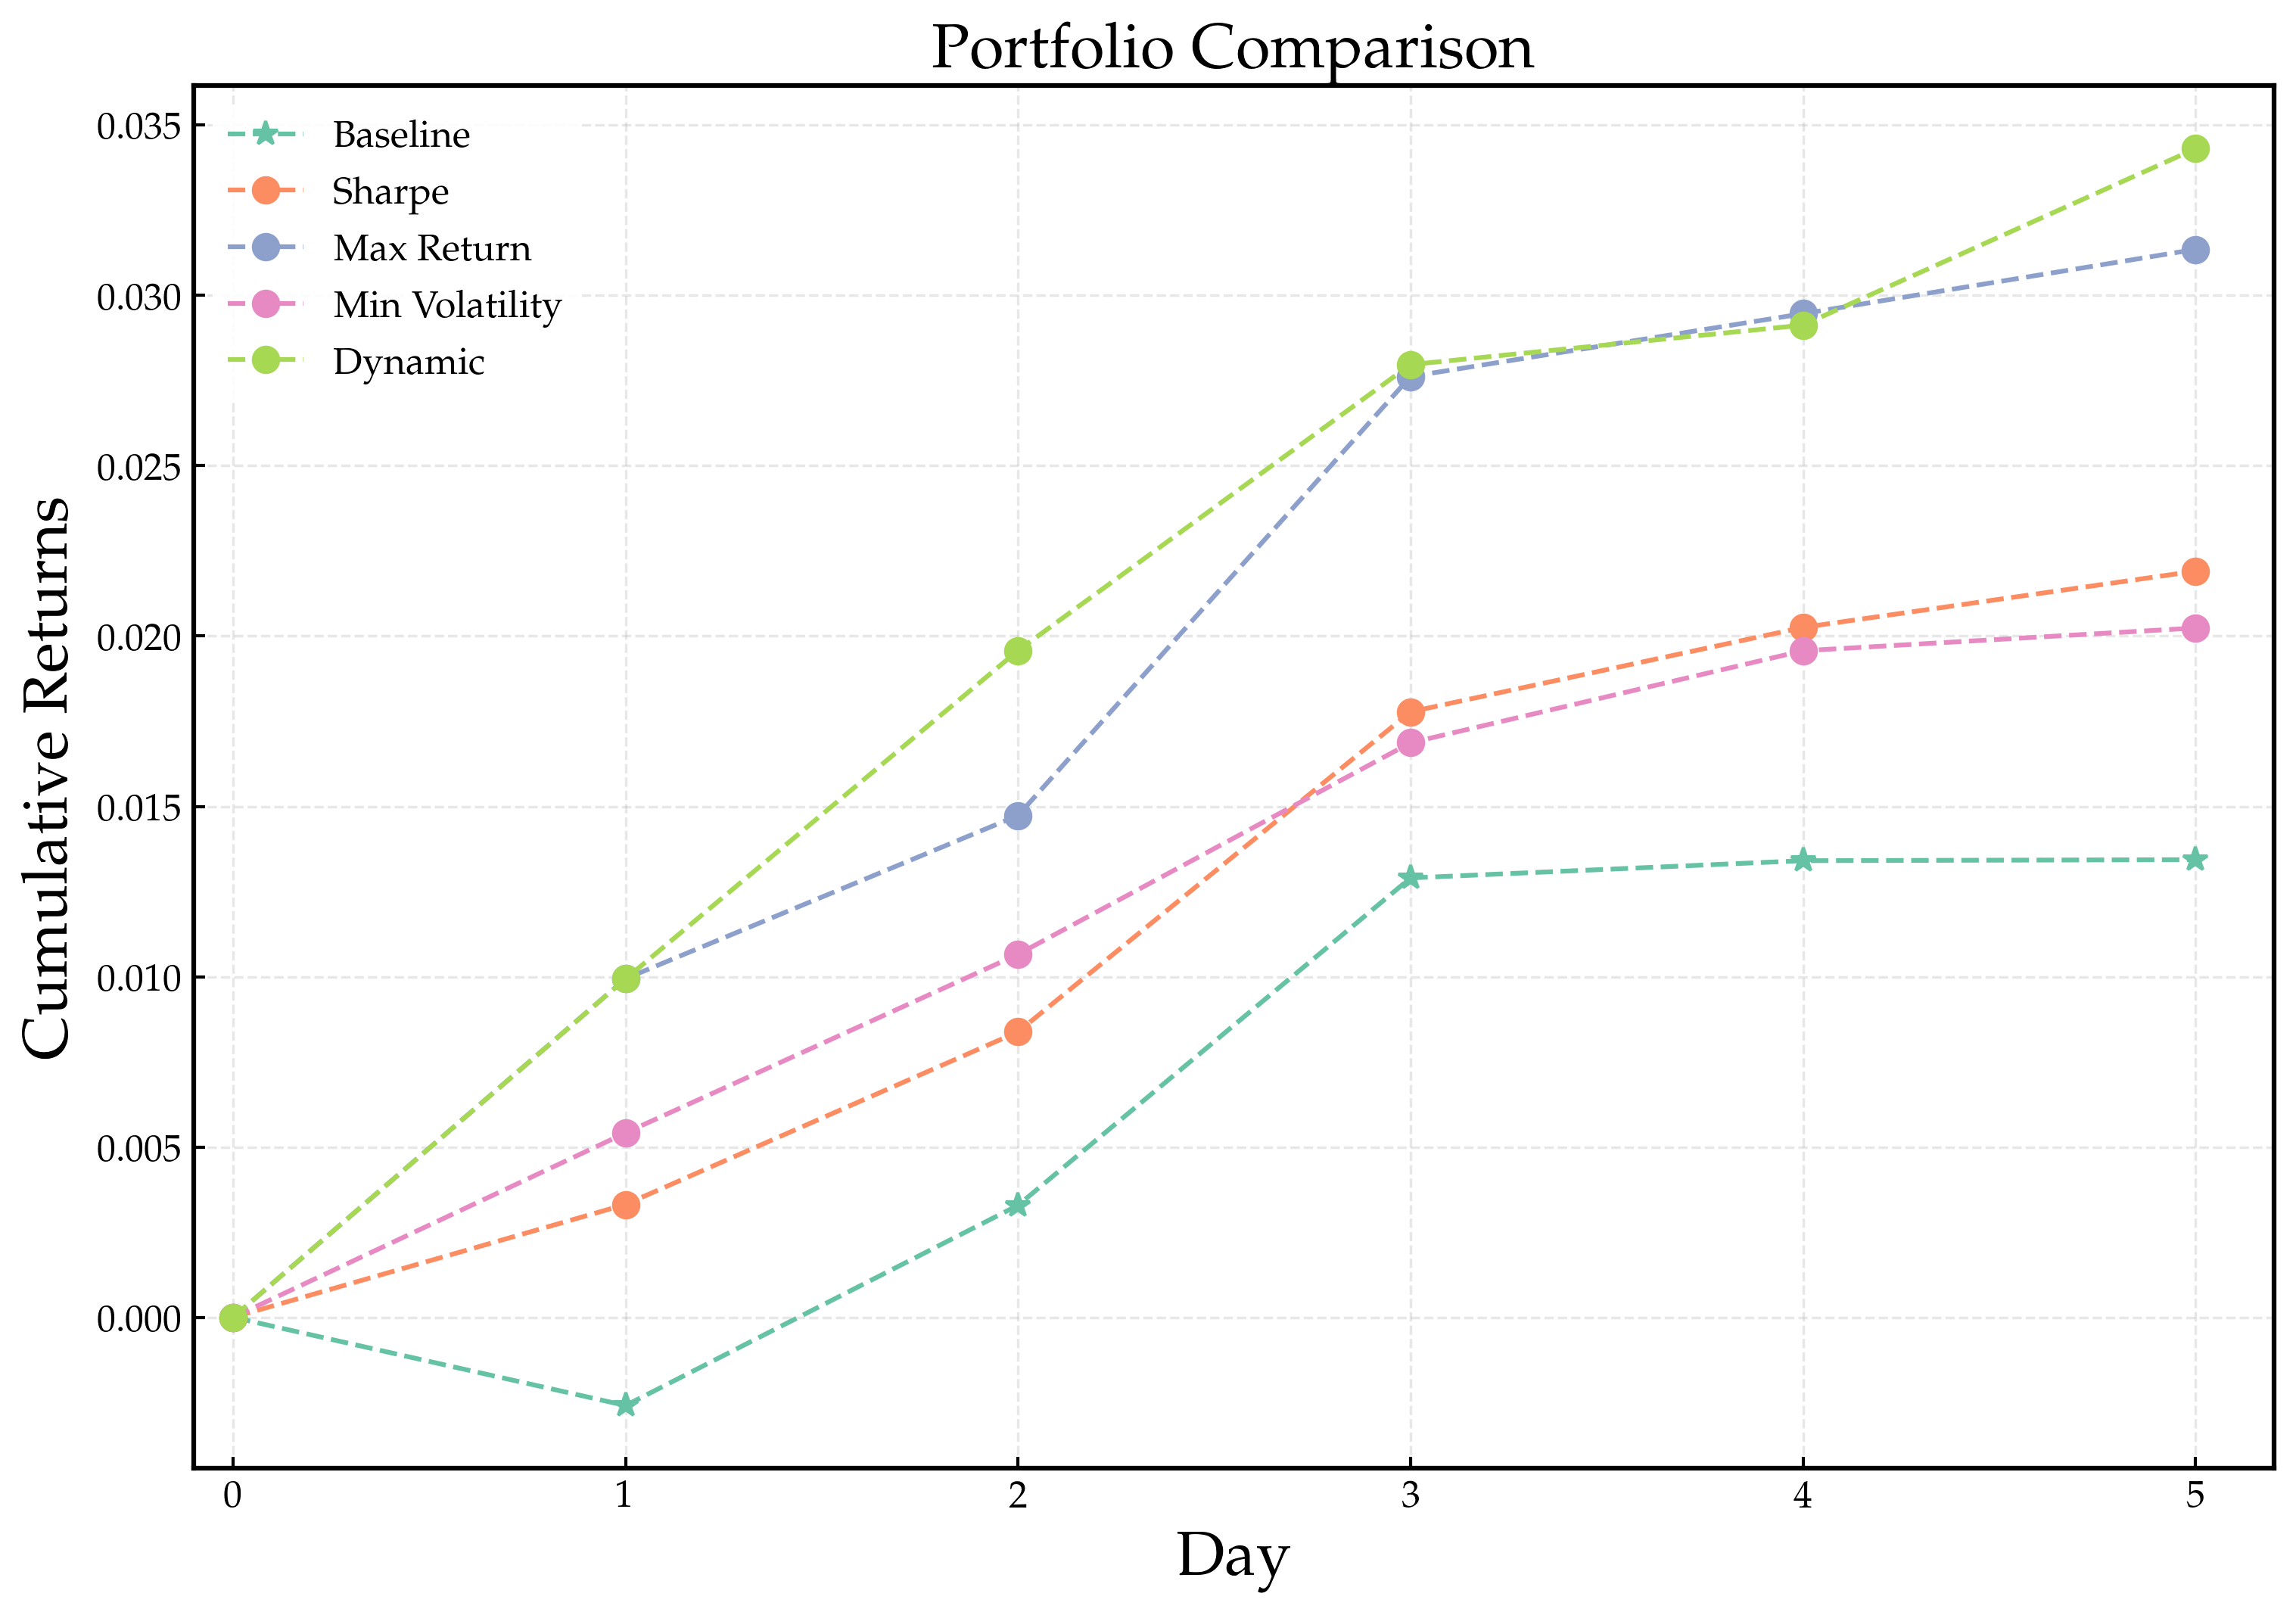
\includegraphics[width=0.6\textwidth]{figures/portfolio_comparison.png}
    \caption{Portfolio Comparison}
    \label{fig:portfolio_comparison}
\end{figure}

Risk metrics
Transaction costs impact

\begin{figure}[h]
    \centering
    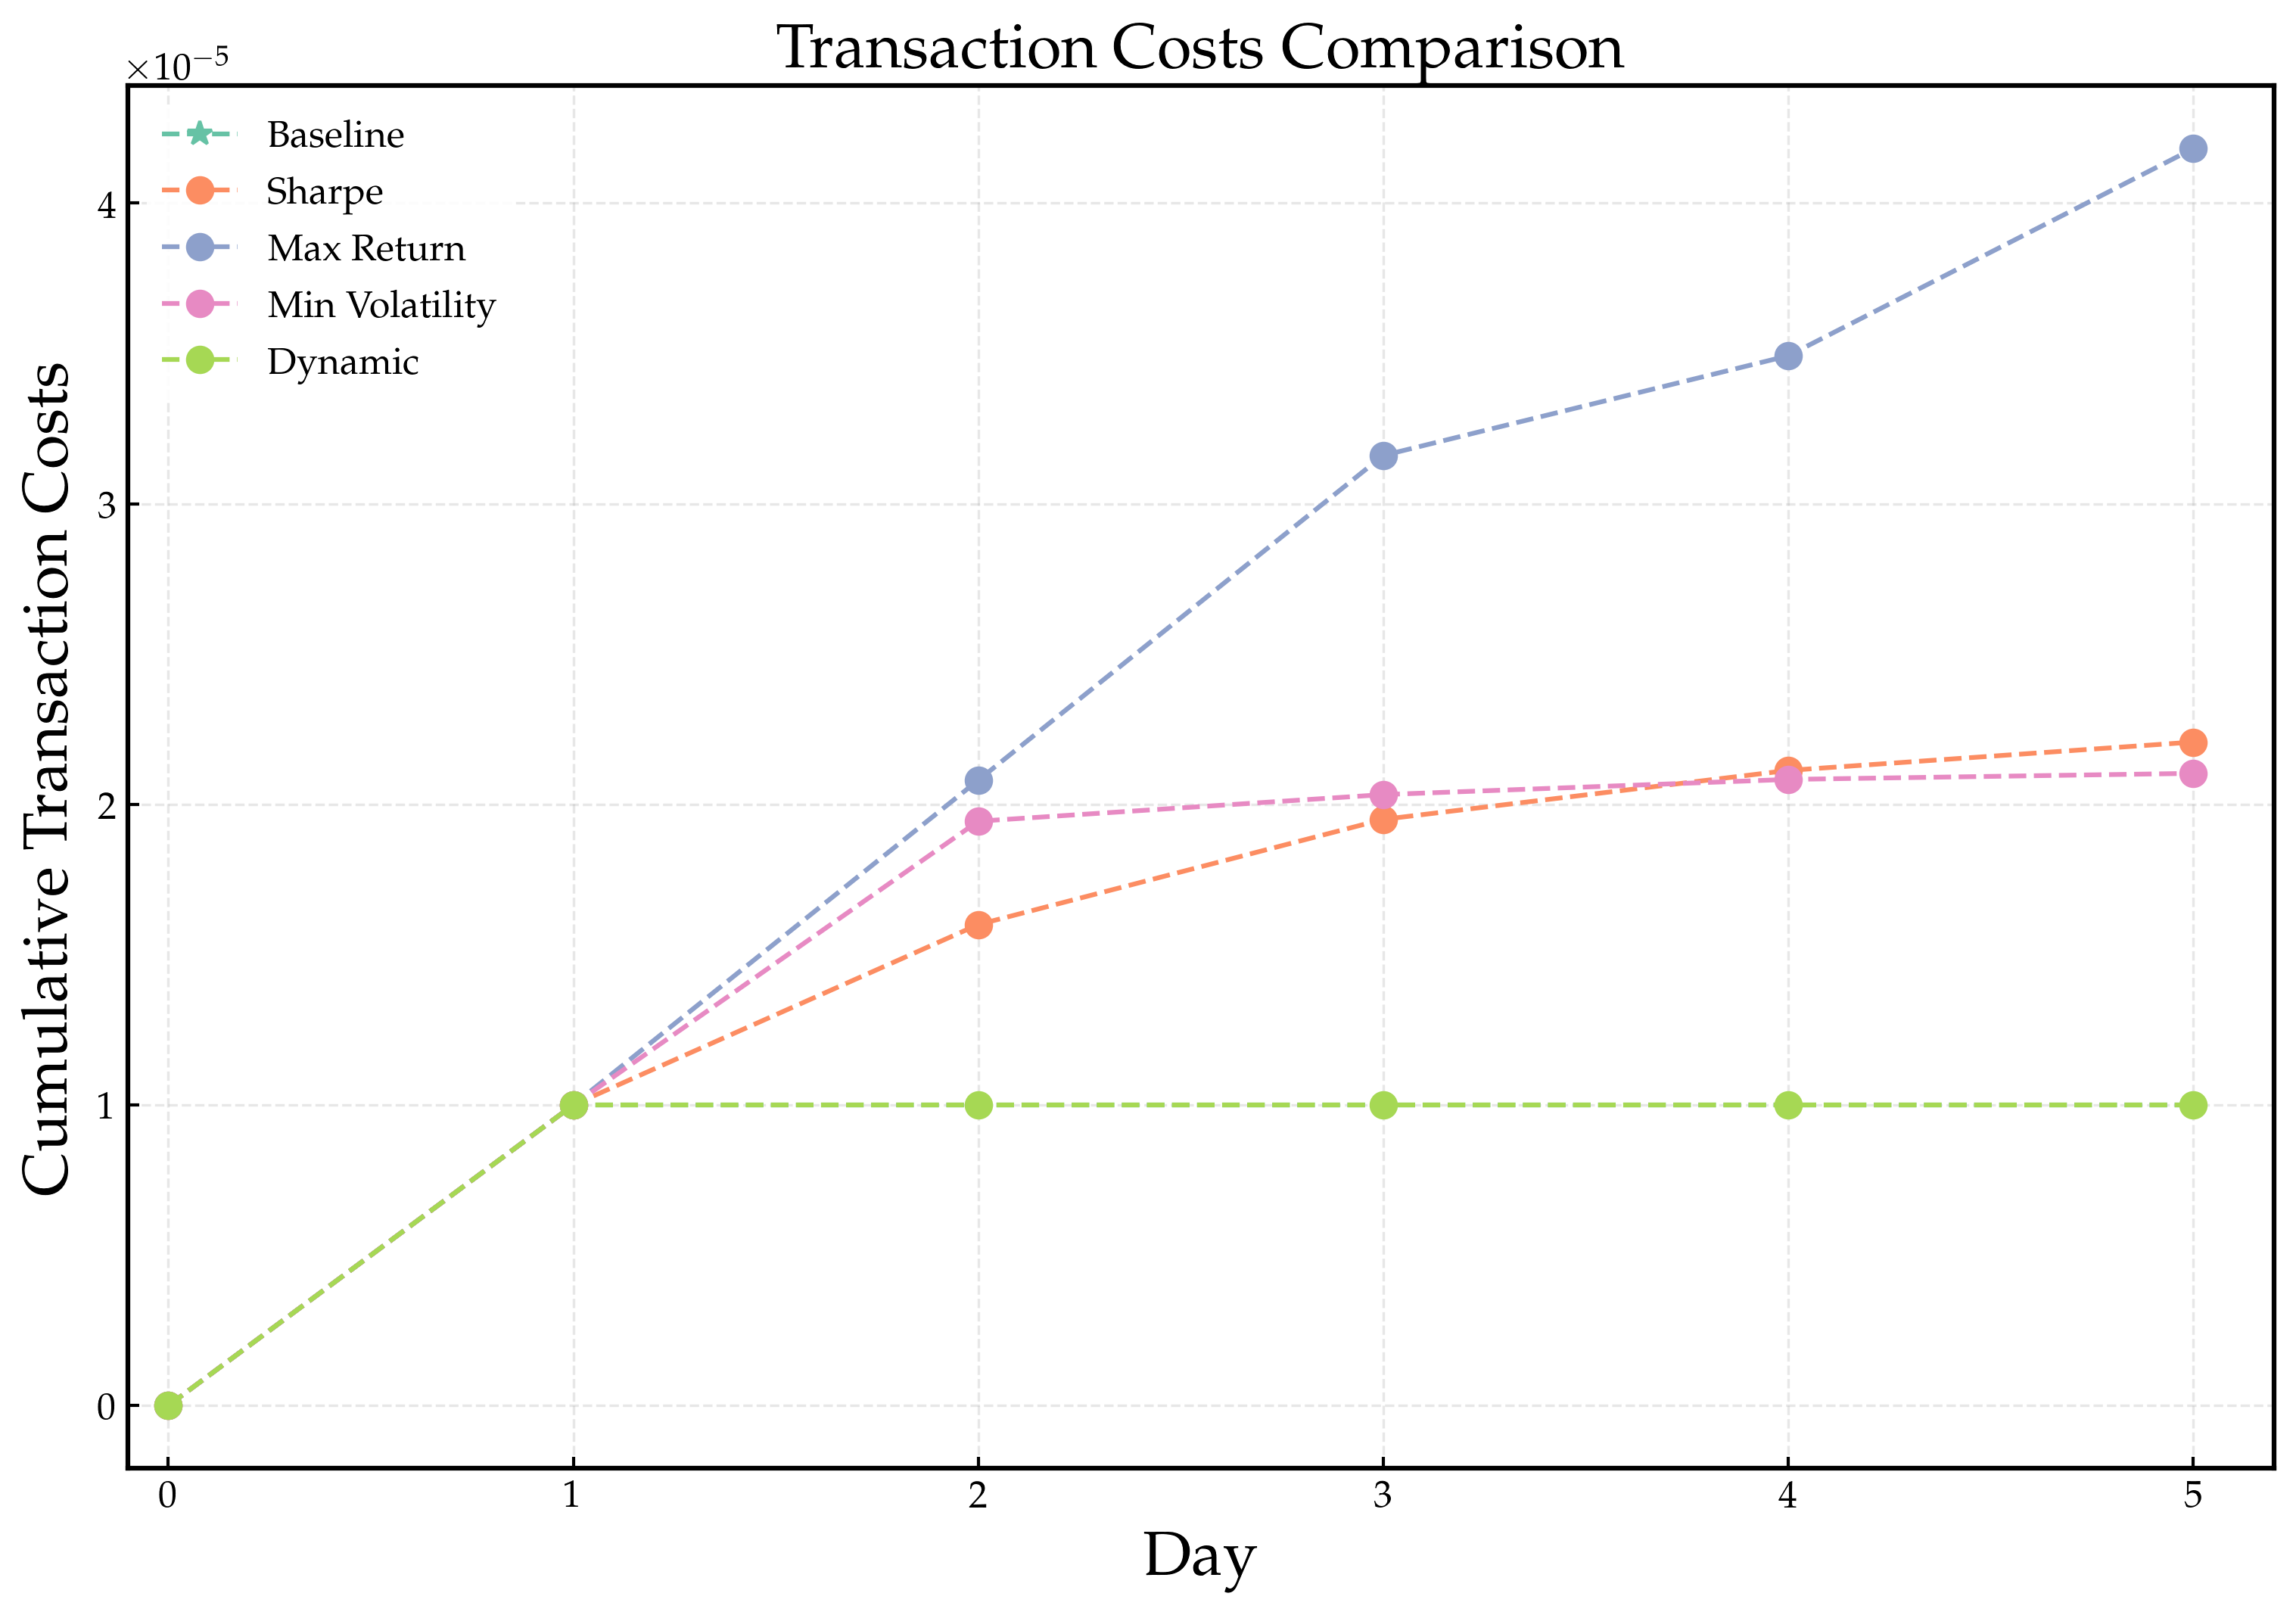
\includegraphics[width=0.6\textwidth]{figures/trx_costs_comparison.png}
    \caption{Transaction Costs Comparison}
    \label{fig:trx_costs_comparison}
\end{figure}

Strategy switching frequency analysis


Comparative Analysis:
Compare the performance of all strategies, highlighting the strengths and weaknesses of each.

\subsection{Dynamic Strategy Evaluation}
Probability threshold sensitivity
Strategy switching effectiveness
Portfolio turnover analysis
Risk-adjusted performance metrics

\section{Backtesting Results}
Provide detailed results from the backtesting, including cumulative returns, volatility, Sharpe ratios, and transaction costs for each strategy.

\subsection{Transaction Costs impact}


\section{Robustness Tests}

\subsection{Different market conditions}

\subsection{Hyperparameter sensitivity}

\subsection{Out-of-sample performance}

\subsection{Statistical significance tests}



% !TeX root = ../main.tex
% Add the above to each chapter to make compiling the PDF easier in some editors.

\chapter{Discussion}\label{chapter:discussion}
The preceding chapters have detailed the methodology, analysis, and results of this research, highlighting the integration of Gaussian Process Regression (GPR) with portfolio optimization strategies. 
This chapter discusses the findings in depth, analyzing their significance, practical implications, and limitations, while outlining opportunities for future research.
\section{Interpretation of Results}
The backtesting results provide critical insights into the performance of various portfolio optimization strategies, particularly the proposed Dynamic Strategy.

\subsection{Key findings and insights}
The Dynamic Strategy, leveraging \ac{GPR}-based predictions, consistently outperformed traditional approaches in terms of risk-adjusted returns. The integration of probabilistic forecasting allowed for dynamic allocation adjustments that were both timely and precise. This was evident in its superior Sharpe Ratio and lower transaction costs compared to other strategies.
While the Maximum Return Strategy delivered higher absolute returns during bull markets, it suffered significant drawdowns during volatile periods. Conversely, the Minimum Volatility Strategy offered stability but lacked responsiveness to high-growth opportunities. The Maximum Sharpe Ratio Strategy balanced these trade-offs, but its static nature limited adaptability in rapidly changing markets.
The \ac{GPR}-enhanced Dynamic Strategy uniquely addressed these limitations by adapting to both upward and downward trends in market conditions, underscoring the value of integrating advanced predictive models in portfolio management.

\subsection{Dynamic Strategy Insights}
The success of the Dynamic Strategy can be attributed to its dual focus on return maximization and risk management. By utilizing GPR’s probabilistic predictions, the strategy dynamically adjusted portfolio allocations based on the predicted distribution of returns and associated uncertainties. This adaptability was particularly effective during transitional market phases, where traditional strategies often falter.
Additionally, the threshold-based decision-making approach minimized unnecessary rebalancing, reducing transaction costs and preserving capital. This efficiency is critical for maintaining net returns, especially in markets characterized by high volatility.

\subsection{Model robustness and generalization}
The \ac{GPR}-based framework demonstrated strong robustness across different market scenarios, highlighting its potential for generalization. The model’s ability to capture non-linear relationships and provide uncertainty quantification was instrumental in adapting to diverse conditions. However, the strategy’s performance was sensitive to the quality of input data and the tuning of hyperparameters, suggesting that further refinements could enhance its reliability and applicability.
\section{Implications for Practitioners}
The findings have several implications for portfolio managers and financial analysts aiming to integrate predictive modeling into their investment strategies.
\subsection{Practical Utility of Dynamic Strategy}
The Dynamic Strategy represents a significant advancement in portfolio optimization by combining predictive analytics with adaptive decision-making. Practitioners can leverage this approach to achieve superior returns while managing risk more effectively. The integration of probabilistic forecasts into the allocation process allows for a nuanced understanding of market conditions, enabling more informed and confident investment decisions.
Moreover, the reduction in transaction costs achieved through threshold-based rebalancing makes the strategy highly practical for real-world application, particularly in environments where high-frequency trading is cost-prohibitive.
\subsection{Limitations of the approach}
Despite its advantages, the GPR-based Dynamic Strategy is not without limitations. The computational complexity of Gaussian Process models can pose challenges for scalability, especially when applied to large portfolios with numerous assets. Additionally, the strategy relies heavily on accurate and timely input data; any deficiencies in data quality or delays in processing can adversely impact performance.
Another practical challenge lies in the interpretability of GPR outputs for non-technical stakeholders. While the model provides robust predictions and uncertainty quantification, translating these insights into actionable strategies requires expertise in both machine learning and finance.

\section{Comparative Analysis}
The comparative evaluation of the strategies provides valuable insights into their relative strengths and weaknesses.


\subsection{Advantages and disadvantages}
The Maximum Return Strategy excels in high-growth markets but exposes investors to significant risks during downturns. Conversely, the Minimum Volatility Strategy offers stability but limits upside potential. The Maximum Sharpe Ratio Strategy strikes a balance but lacks the adaptability required for dynamic environments.
The Dynamic Strategy stands out by addressing these limitations through its adaptability and efficiency. However, its reliance on sophisticated models introduces complexity that may not be suitable for all investors.
\subsection{Implementation challenges}
Implementing the Dynamic Strategy requires a robust computational infrastructure and access to high-quality data. Additionally, portfolio managers must account for regulatory and operational constraints, such as compliance with trading limits and reporting requirements.
\subsection{Market impact considerations}

The strategy's dynamic nature raises considerations regarding market impact, particularly in illiquid markets where frequent rebalancing could influence asset prices. Future research should explore ways to mitigate such effects while maintaining strategy effectiveness.

\section{Future Research Directions}

\subsection{Model Improvements}
While the Gaussian Process Regression (GPR) model has demonstrated robust predictive capabilities, there are several areas where its performance and applicability in financial markets could be enhanced. 
One significant opportunity lies in kernel optimization and design, espeically given the circumestance that we eventually only chose to use Exponential Kernels as it performed the best out of all the standard common kernels.
By exploring custom kernel functions tailored specifically for financial time-series data, it would be possible to better capture the unique characteristics of market dynamics. 
For example, kernels designed to explicitly model long-range dependencies or volatility clustering could provide more accurate predictions. 
Additionally, multi-kernel approaches that combine different kernel types might offer greater flexibility, enabling the model to simultaneously account for short-term fluctuations and long-term trends.

Another promising avenue for improvement is the incorporation of multi-output predictions. 
Extending GPR to forecast multiple correlated outputs—such as returns of assets within the same sector—could deepen the model's ability to understand and leverage interdependencies between assets. 
This approach could be facilitated by employing multi-task learning frameworks, which enable the simultaneous prediction of related outputs.

Integrating macroeconomic indicators into the GPR framework is another enhancement that could significantly improve its forecasting accuracy. 
Variables such as GDP growth, inflation rates, or central bank policy signals provide valuable contextual information that influences market trends. 
By including these indicators, the model could generate predictions that are not only more accurate but also more responsive to broader economic conditions.

Addressing non-stationarity in financial time-series data is also critical for improving GPR's applicability. 
Financial markets are characterized by trends, regime changes, and abrupt shifts, all of which violate the assumption of stationarity in standard GPR implementations. 
Techniques such as change-point detection, which segments the data into stationary intervals, or the incorporation of non-stationary covariance structures, could help the model better adapt to these complexities.


Finally, computational efficiency remains a key area for enhancement, particularly for real-time applications and large portfolios. 
GPR's computational complexity, which grows with the size of the dataset, can be mitigated using methods such as sparse Gaussian Process approximations, inducing points, or scalable variants like stochastic variational GPs. 
These techniques could enable the model to handle larger datasets and deliver faster predictions, making it more practical for real-world financial decision-making. 
By addressing these areas, GPR can be further refined to meet the demands of complex and dynamic financial environments.

\subsubsection{Composite \ac{GPR} Model for Multi-Scale Forecasting}
Specifically, we proposed a composite Gaussian Process Regression (GPR) model that effectively integrates short-term (daily), mid-term (weekly), and long-term (monthly) stock price data to improve predictive accuracy. 
The integration of multiple time scales captures unique patterns and trends from different temporal resolutions, providing a holistic view of market dynamics. 
By combining these diverse data sources, the model leverages the strengths of each time scale, enhancing its adaptability and robustness.

The optimization objective is formulated as:
\[
\min_{\alpha, \beta} \quad L(\alpha, \beta) = \text{MSE}\left(Y, \hat{f}_{\text{combined}}\right) + \lambda \left( |\alpha| + |\beta| \right)
\]

where:
\begin{itemize}
    \item $L(\alpha, \beta)$: The loss function, which balances the mean squared error (MSE) of predictions with an $L_1$-regularization term to prevent overfitting.
    \item $\hat{f}_{\text{combined}}$: The combined predictive output derived from weighted contributions of daily, weekly, and monthly data.
    \item $\lambda$: A regularization parameter that controls the penalty for large weights, encouraging sparsity in the contributions from different time scales.
\end{itemize}

The combined forecast is given by:

\[
\hat{f}_{\text{combined}} = \alpha \cdot f_{\text{mean,daily}} + \beta \cdot f_{\text{mean,weekly}} + (1 - \alpha - \beta) \cdot f_{\text{mean,monthly}}
\]

where:
\begin{itemize}
    \item $f_{\text{mean,daily}}$: The mean prediction from the daily GPR model.
    \item $f_{\text{mean,weekly}}$: The mean prediction from the weekly GPR model.
    \item $f_{\text{mean,monthly}}$: The mean prediction from the monthly GPR model.
    \item $\alpha, \beta$: Weights assigned to daily and weekly data, respectively. The remaining weight, $1 - \alpha - \beta$, is allocated to the monthly data.
\end{itemize}

\subsubsection*{Constraints}
To ensure stability and interpretability of the model, the following constraints are imposed on the weights:

\[
\begin{cases}
0 \leq \alpha \leq 1 \\
0 \leq \beta \leq 1 \\
\alpha + \beta \leq 1
\end{cases}
\]

These constraints ensure that the weights are non-negative and their sum does not exceed 1, maintaining a probabilistic interpretation of the contributions from each time scale.

\subsection{Additional Strategy Considerations}
Building on the strategies explored in this study, there are numerous opportunities to enhance and diversify approaches to better align with a range of market conditions. One promising modification involves the development of factor-based dynamic strategies. By combining GPR predictions with established factor models such as momentum or value, it is possible to create hybrid strategies that adapt not only to macroeconomic cycles but also to specific factor-driven opportunities. For example, during periods of economic expansion, the strategy could tilt toward value stocks identified through GPR forecasts, while momentum factors might be prioritized during market uptrends.

Another avenue for improvement lies in integrating GPR predictions into risk-parity strategies. These strategies, which aim to balance the risk contributions of assets within a portfolio, could benefit from GPR's ability to predict volatility dynamically. By adjusting risk-parity allocations based on real-time volatility forecasts, the strategy could better respond to evolving market dynamics and maintain a balanced risk profile.

Threshold-based rebalancing approaches could also be enhanced by introducing conditional adjustments. For instance, thresholds could be tightened during periods of high market volatility to ensure that the portfolio remains closely aligned with its target allocation, while wider thresholds could be used during more stable conditions to minimize transaction costs. This dynamic adjustment of thresholds would enable the strategy to adapt more effectively to changing market conditions.

Long-short portfolio strategies represent another area for exploration. By leveraging GPR to identify both predicted outperformers and underperformers, a long-short strategy could capitalize on relative performance differences between assets. This approach is particularly advantageous in neutral or bearish markets, where generating alpha through relative value opportunities becomes more critical.

Lastly, the incorporation of hedging strategies using derivatives such as options or futures could provide additional protection against extreme risks predicted by GPR. For example, when GPR forecasts heightened uncertainty or the potential for significant drawdowns, the portfolio could employ options-based hedges to mitigate downside risks while maintaining exposure to upside potential. This integration of predictive modeling with hedging tools would create a more resilient strategy capable of weathering adverse market conditions.

By pursuing these modifications and new strategies, portfolio managers can better harness the power of GPR to develop adaptive, robust, and highly tailored investment approaches that address the challenges and opportunities of diverse market environments.

\subsection{Alternative Applications}
The methodologies developed in this study extend far beyond traditional portfolio optimization, offering potential applications in various domains where predictive accuracy and uncertainty quantification are critical.

One such application is in risk management systems, where real-time risk monitoring could leverage Gaussian Process Regression (GPR) to forecast market volatility and potential drawdowns. By providing timely and actionable alerts, these systems can enable financial institutions to take preemptive measures, reducing exposure to adverse market conditions and improving overall risk control.

GPR's capability to model non-linear relationships and account for uncertainties also makes it a valuable tool in credit scoring models. For borrowers with limited credit histories or unconventional financial profiles, traditional models often fail to provide accurate risk assessments. \ac{GPR}'s flexibility allows it to incorporate a wider range of variables and generate more nuanced creditworthiness predictions, making it particularly beneficial in underserved markets.

In the realm of algorithmic trading, GPR can guide trading systems by forecasting short-term price movements with precision. These predictions enable dynamic adjustments to trade execution strategies, optimizing entry and exit points based on real-time market conditions. This application is especially relevant in high-frequency trading, where slight improvements in prediction accuracy can yield substantial financial gains.

The methodologies could also be extended to macroeconomic forecasting, where GPR could predict key economic indicators such as unemployment rates, consumer confidence, or inflation. Policymakers and financial analysts could use these forecasts to make informed decisions, improving the accuracy of policy interventions or market predictions.

Another promising area of application is renewable energy forecasting. Given the influence of weather conditions on renewable energy outputs, GPR can model and predict these fluctuations, aiding energy traders and utility companies in balancing supply and demand \cite{en13205509}. This capability would improve efficiency in energy markets and support the transition to sustainable energy systems.

Lastly, GPR can play a vital role in ESG (Environmental, Social, and Governance) and impact investing by forecasting ESG-related metrics. By providing reliable predictions on factors such as carbon emissions, social impact scores, or governance indicators, GPR enables investors to align their portfolios with sustainability objectives. This alignment is increasingly important in meeting the growing demand for socially responsible investment strategies.

These alternative applications demonstrate the versatility of GPR and its potential to drive innovation and efficiency across a wide array of industries, making it a valuable tool not just for portfolio optimization but for addressing broader challenges in risk management, trading, forecasting, and sustainability.

\subsection{Scalability Considerations}
Scalability is a crucial factor for implementing Gaussian Process Regression (GPR) in large-scale portfolios or real-time applications, where computational efficiency and responsiveness are paramount. To address these challenges, several strategies can enhance the model's scalability while maintaining accuracy and reliability.

One critical component is the implementation of efficient data processing pipelines. Utilizing parallelized frameworks such as Apache Spark or Dask can streamline data preprocessing, training, and prediction execution, enabling near real-time operations. These tools allow for the handling of large datasets by distributing computational tasks across multiple nodes, significantly reducing processing times.

Sparse Gaussian Processes (GPs) present another effective solution. By employing techniques such as inducing points, sparse GPs reduce the computational complexity associated with traditional GPR, making it feasible to work with large datasets without excessive resource consumption. This approach approximates the full GPR while preserving its core predictive capabilities.

Hierarchical modeling offers an additional avenue to enhance scalability. By grouping assets based on sectors, regions, or other logical categories and applying GPR within these clusters, the complexity of covariance estimation is significantly reduced. This hierarchical approach not only simplifies the computation but also maintains accuracy by tailoring predictions to specific subsets of the portfolio.

For real-time applications, edge computing provides a practical solution to reduce latency. Deploying GPR models on edge devices, such as servers located closer to trading platforms or risk management systems, ensures faster response times. This approach is particularly beneficial for high-frequency trading or dynamic risk monitoring, where delays can result in missed opportunities or increased exposure \cite{Doe2021}.

Cloud-based scalability further complements these solutions by leveraging platforms such as AWS SageMaker or Google Vertex AI. These platforms offer on-demand scaling of computational resources, allowing GPR models to handle fluctuating workloads efficiently. Additionally, they support real-time data ingestion and model deployment, ensuring that the system can adapt to evolving market conditions without manual intervention.

Lastly, integrating alternative data sources, such as satellite imagery, social media sentiment, or web scraping outputs, can enrich GPR's input features, enhancing its predictive power. However, incorporating such diverse data types requires robust preprocessing and scalable storage solutions. Distributed databases and cloud-based architectures can ensure that these non-traditional data sources are processed efficiently and seamlessly integrated into the modeling pipeline.

By adopting these strategies, GPR can be scaled effectively for large portfolios and real-time applications, providing accurate and timely predictions without compromising computational efficiency or resource availability. These considerations are essential for extending the practical utility of GPR in modern financial systems.









% !TeX root = ../main.tex
% Add the above to each chapter to make compiling the PDF easier in some editors.

\chapter{Conclusion}\label{chapter:conclusion}

\section{Summary of Findings}
\subsection{Summary of Findings}
Recap the main results and how they address your research questions.
\subsection{Key findings and insights}
Discuss what the results mean in the context of your research objectives.

\section{Recommendations}
Offer suggestions for practitioners based on your findings.

\section{Future Research Directions}


\subsection{Model improvements}
Discuss potential enhancements to your model or methodology.

\subsection{Additional strategy considerations}
Suggest new strategies or modifications to existing ones.

\subsection{Alternative applications}
Propose other areas where your approach could be useful.
\subsection{Scalability considerations}







\appendix{}

\microtypesetup{protrusion=false}

\addchap{Abbreviations}
\begin{acronym}
	\itemsep-.25\baselineskip
	\acro{TUM}[TUM]{Technical University of Munich}
	\acro{GPR}[GPR]{Gaussian Processes Regression}
	\acro{GP}[GP]{Gaussian Processes}
	\acro{ML}[ML]{Machine Learning}
	\acro{MSE}[MSE]{Mean Squared Error}
	\acro{RMSE}[RMSE]{Root Mean Squared Error}
	\acro{MAE}[MAE]{Mean Absolute Error}
	\acro{SVM}[SVM]{Support Vector Machine}
	\acro{ANN}[ANN]{Artificial Neural Network}
	\acro{RBF}[RBF]{Radial Basis Function}
	\acro{LSTM}[LSTM]{Long Short-Term Memory}
	\acro{GRU}[GRU]{Gated Recurrent Unit}
	\acro{RNN}[RNN]{Recurrent Neural Network}
	\acro{ARIMA}[ARIMA]{AutoRegressive Integrated Moving Average}
	\acro{VAR}[VAR]{Vector AutoRegressive}
	\acro{MPT}[MPT]{Modern Portfolio Theory}
	% TODO: add acronyms
\end{acronym}


\listoffigures{}
\listoftables{}
\microtypesetup{protrusion=true}
\printbibliography{}

\end{document}
